\documentclass[11pt]{amsart}

\usepackage[utf8]{inputenc}
\usepackage{upquote}
\usepackage{amssymb}
\usepackage[margin=1in]{geometry}
\usepackage{enumitem}
\usepackage{tikz}
\usepackage{booktabs}
\usepackage{longtable}
\usepackage{array}
\usepackage[hidelinks]{hyperref}

% Unicode characters used in the Lean excerpt of Section 8
\DeclareUnicodeCharacter{2115}{\ensuremath{\mathbb{N}}}
\DeclareUnicodeCharacter{2203}{\ensuremath{\exists}}
\DeclareUnicodeCharacter{2200}{\ensuremath{\forall}}
\DeclareUnicodeCharacter{2194}{\ensuremath{\leftrightarrow}}
\DeclareUnicodeCharacter{2192}{\ensuremath{\to}}
\DeclareUnicodeCharacter{2209}{\ensuremath{\notin}}
\DeclareUnicodeCharacter{2227}{\ensuremath{\wedge}}
\DeclareUnicodeCharacter{2264}{\ensuremath{\le}}
\DeclareUnicodeCharacter{2243}{\ensuremath{\simeq}}

\newtheorem{theorem}{Theorem}[section]
\newtheorem{lemma}[theorem]{Lemma}
\newtheorem{proposition}[theorem]{Proposition}
\newtheorem{corollary}[theorem]{Corollary}
\theoremstyle{definition}
\newtheorem{definition}[theorem]{Definition}
\newtheorem{example}[theorem]{Example}
\newtheorem{question}[theorem]{Question}
\theoremstyle{remark}
\newtheorem{remark}[theorem]{Remark}

\newcommand{\Lam}{\Lambda}
\newcommand{\Tr}[1]{T(#1)}
\newcommand{\D}{\mathcal{D}}
\newcommand{\cl}{\operatorname{cl}}
\newcommand{\intr}{\operatorname{int}}
\newcommand{\doi}[1]{\href{https://doi.org/#1}{doi:\nolinkurl{#1}}}
\newcommand{\arXiv}[1]{\href{https://arxiv.org/abs/#1}{arXiv:\nolinkurl{#1}}}
\newcommand{\grepo}{\url{https://github.com/LucasAlves8Sp/THE-INVERSE-PROBLEM-FOR-THE-NUMBER-OF-CONNECTED-INDUCED-SUBGRAPHS}}
\newcommand{\repo}{\url{https://github.com/LucasAlves8Sp/ALL-FINITE-CARDINALITIES-OF-THE-HYPERSPACE-OF-REGULAR-SUBCONTINUA}}

\begin{document}

\title[The number of connected induced subgraphs]{The inverse problem for the number of\\ connected induced subgraphs}

\author{Lucas Alves de Almeida}
\address{Independent researcher}
\email{lucasderiva8x@gmail.com}

\date{November 2026}

\subjclass[2020]{Primary 05C30; Secondary 05C40, 54B20, 68V20}

\keywords{Connected induced subgraph, connected set, inverse problem, graph invariant, subtrees, cone, formal verification, Lean}

\begin{abstract}
For a finite graph $G$, let $c(G)$ be the number of nonempty vertex sets that induce a connected subgraph. We show that a positive integer $k$ equals $c(G)$ for some finite connected graph $G$ if and only if $k\notin\{2,4,5,8,9,16\}$. Every attainable value $k\ne25$ is attained on $\lfloor\log_2k\rfloor+1$ vertices, the least possible number, and $25$ needs six vertices. More precisely, for every $m\ge6$ each integer from $2^{m-1}$ to $2^m-1$ is the value of $c$ on a connected graph with exactly $m$ vertices. The proofs of these results are short and use no computer; computer calculations serve only as independent checks, and for two auxiliary results: the values on six to eight vertices, and the result on all connected subgraphs described below. The value $16$ falls into a gap above the path: a connected graph on $n\ge4$ vertices other than the path $P_n$ has at least $n-3$ more connected sets than $P_n$. The values $k\ge17$ are realized by a recursive construction from cones, disjoint unions and a family of graphs that we call near-cones, starting from seven small graphs; it produces a graph with $c(G)=k$ in time polynomial in $\log k$. The question arose from a problem of Ordo\~nez in continuum theory, through a reduction by Camargo, Ordo\~nez and Ram\'irez, who found the values up to $255$ by a computer search. The proof is formalized in Lean~4. We also observe that a theorem of Czabarka, Sz\'ekely and Wagner on subtrees reduces the corresponding problem for the number of all connected subgraphs to a finite computation, and we report its outcome. We did not find these results in the literature, but we make no claim of novelty or priority.
\end{abstract}

\maketitle

\section{Introduction}\label{sec:intro}

Let $G$ be a finite simple graph. A \emph{connected set} of $G$ is a nonempty set of vertices that induces a connected subgraph, and $c(G)$ denotes the number of connected sets of $G$. Equivalently, $c(G)$ is the number of connected induced subgraphs of $G$, where subgraphs induced by different vertex sets are counted separately even when they are isomorphic. For instance,
\[
c(P_n)=\frac{n(n+1)}2,\qquad c(K_n)=2^n-1,\qquad c(K_{1,d})=2^d+d,\qquad c(C_n)=n(n-1)+1
\]
for the path, the complete graph, the star and the cycle; these and several other closed formulas are given by Vince \cite[Example~1]{Vi}. For a tree, $c(G)$ is the number of subtrees. Write $\Tr{n}=n(n+1)/2$. If $G$ is connected with $n$ vertices, then
\begin{equation}\label{eq:range}
\Tr{n}\le c(G)\le 2^n-1
\end{equation}
(Lemma~\ref{lem:rules}(f)). The \emph{inverse problem} for $c$ asks which positive integers are of the form $c(G)$. The question is only interesting for connected graphs: $c$ is additive over components, so every positive integer $k$ is $c$ of the edgeless graph on $k$ vertices.

\begin{theorem}\label{thm:main}
A positive integer $k$ equals $c(G)$ for some finite connected graph $G$ if and only if
\[
k\notin\{2,4,5,8,9,16\}.
\]
\end{theorem}

The upper bound in \eqref{eq:range} shows that a connected graph with $c(G)=k$ has at least $\lfloor\log_2k\rfloor+1$ vertices. This bound is attained with a single exception.

\begin{theorem}\label{thm:order}
Let $k$ be a positive integer with $k\notin\{2,4,5,8,9,16\}$. The least number of vertices of a connected graph $G$ with $c(G)=k$ is $\lfloor\log_2k\rfloor+1$ if $k\ne25$, and $6$ if $k=25$.
\end{theorem}

Both theorems follow from a statement about graphs with a prescribed number of vertices. For $m\ge0$ let
\begin{align*}
V_m&=\{c(G): G\text{ a connected graph with exactly }m\text{ vertices}\},\\
\Lam_m&=\{c(G): G\text{ a graph with exactly }m\text{ vertices}\}.
\end{align*}
For integers $a\le b$ we write $[a,b]=\{a,a+1,\dots,b\}$. By \eqref{eq:range}, $V_m\subseteq[\Tr{m},2^m-1]$.

\begin{theorem}\label{thm:dyadic-intro}
\begin{enumerate}[label=\textup{(\alph*)}]
\item For every $m\ge6$, $V_m\supseteq[2^{m-1},2^m-1]$: every integer $k$ with $2^{m-1}\le k\le 2^m-1$ is $c(G)$ for a connected graph $G$ with exactly $m$ vertices.
\item For every $m\ge7$, $\Lam_m\supseteq[m,2^m-1]$.
\end{enumerate}
\end{theorem}

Part (a) fails for $m=5$, since $25\notin V_5$ (Proposition~\ref{prop:V5}). A computer search shows that part (b) fails for $m=6$, since $26\notin\Lam_6$ (Section~\ref{sec:computation}).

\emph{Where the exceptions come from.} By \eqref{eq:range}, the values of $c$ on connected graphs with $n=1,2,3,4,5,6$ vertices lie in the intervals
\[
[1,1],\quad[3,3],\quad[6,7],\quad[10,15],\quad[15,31],\quad[21,63],
\]
and from $n=4$ on consecutive intervals overlap. The five integers $2,4,5,8,9$ lie in none of these intervals. The integer $16$ lies only in the interval for $n=5$, and there it equals $\Tr{5}+1$. It falls into a gap just above the path. A connected graph on $n\ge4$ vertices other than $P_n$ has at least $\Tr{n}+n-3$ connected sets (Proposition~\ref{prop:pathgap}), so $\Tr{n}+1,\dots,\Tr{n}+n-4$ are never attained on $n$ vertices. For $n\ge6$ these gaps are covered by graphs with fewer vertices, but for $n=5$ the gap is the single value $16$, and no other order covers it. Theorems~\ref{thm:main}--\ref{thm:dyadic-intro} say that nothing else is lost.

\emph{The method.} The proofs of Theorems~\ref{thm:main}--\ref{thm:dyadic-intro} use no computer. Computer calculations appear in this paper only as independent checks of explicit counts (Section~\ref{sec:computation}), in the census of the values on six to eight vertices (Section~\ref{sec:fixed}), and in Proposition~\ref{prop:F} on all connected subgraphs, which is labelled as computer-assisted. The exclusions come from \eqref{eq:range} and Proposition~\ref{prop:pathgap}. For the realizations, the basic observation is that adding a universal vertex to a graph $K$ (taking the \emph{cone} over $K$) adds exactly $2^{|K|}$ connected sets. So the cones over the graphs with $m-1$ vertices realize $2^{m-1}+\Lam_{m-1}$ on $m$ vertices. Every graph on $m-1$ vertices has at least $m-1$ connected sets, so cones miss the $m-1$ values at the bottom of $[2^{m-1},2^m-1]$. To fill this gap we use \emph{near-cones} (Definition~\ref{def:nearcone}). A near-cone is the cone over the disjoint union of a star and a graph $R$, with one edge at the apex removed; removing that edge destroys exactly $2^{|R|}$ connected sets. Choosing the size of the star near $\log_2m$ makes the missing values reachable from $\Lam_{|R|}$ by induction (Theorem~\ref{thm:dyadic}). The induction starts at seven vertices and needs seven small graphs, which we call \emph{sporadic}. The construction is explicit and yields a graph with $c(G)=k$ on $\lfloor\log_2k\rfloor+1$ vertices in time polynomial in $\log k$ (Remark~\ref{rem:algorithm}).

\subsection{How the problem arose}\label{subsec:origin}

This work started from a question in continuum theory. A \emph{continuum} is a nonempty compact connected metric space. A subcontinuum $A$ of a continuum $X$ is \emph{regular} if $A=\cl_X\intr_XA$, and Ordo\~nez \cite{Or18} introduced the hyperspace $\D(X)$ of regular subcontinua of $X$. He asked for which $n$ there is a continuum $X$ with exactly $n$ regular subcontinua \cite[Problem~4.14]{Or18}. Camargo, Ordo\~nez and Ram\'irez \cite{CORa} showed that when $\D(X)$ is finite, it is determined by its minimal elements, which have pairwise disjoint interiors and cover $X$ \cite[Theorem~3.16]{CORa}. This reduces the computation of $|\D(X)|$ to a count in a graph: $|\D(X)|$ is the number of connected sets of the intersection graph of these minimal elements, a finite connected graph \cite{CORa}, \cite[Proposition~3.2]{AA2}. They proved that $|\D(X)|\notin\{2,4,5,8,9\}$ \cite[Proposition~3.18]{CORa}. A computer search over all graphs with at most eight vertices showed that $16$ does not occur as a value of $c$, while every integer from $17$ to $255$ does \cite[Remark~3.20]{CORa}. They asked whether every $k\ge256$ is the cardinality of some $\D(X)$ \cite[Question~3.21]{CORa}.

The author was working on this question. In a companion paper \cite{AA2} we answer it: the finite cardinalities of $\D(X)$ are exactly the positive integers outside $\{2,4,5,8,9,16\}$. That paper realizes every finite connected graph by copies of the Knaster continuum glued at points. Hence the topological question is equivalent to the graph-theoretic one, which is Theorem~\ref{thm:main}. The graph-theoretic result does not depend on continuum theory and may be of independent interest. So we present it here on its own, with complete proofs and a more detailed explanation of the construction. Compared with \cite{AA2}, this paper also contains a new and more conceptual treatment of five vertices (Propositions~\ref{prop:pathgap} and~\ref{prop:V5}) and some related observations (Sections~\ref{sec:fixed} and~\ref{sec:related}).

\subsection{Related work and the status of the result}\label{subsec:literature}

The invariant $c(G)$ has been studied mainly from the extremal point of view. For trees, $c$ is the number of subtrees, studied by Sz\'ekely and Wang \cite{SW}, among others. For general graphs, Dossou-Olory \cite{DO1,DO2,DO3}, Andriantiana and Dossou-Olory \cite{ADO} (Nordhaus--Gaddum inequalities), and Haslegrave \cite{Ha} studied the extremal values of $c$ and of related counts of connected sets. Vince \cite{Vi} studied the growth of $c$, and of the number of partitions of the vertex set into connected sets, along infinite families of graphs; he computed $c$ for several families and bounded it in terms of the number of edges. The invariant is a specialization of the subgraph component polynomial of Tittmann, Averbouch and Makowsky \cite{TAM}, which counts vertex sets by their size and by the number of components of the induced subgraph; $c(G)$ counts the vertex sets inducing exactly one component. Pandey and Patra \cite{PP} studied extremal problems for the number $F(G)$ of all connected subgraphs, not necessarily induced.

Inverse problems ask which values a graph invariant takes. Linek \cite{Li} showed that every positive integer is the number of independent sets of a bipartite graph. Wang and Yu \cite{WY} showed that all but $49$ positive integers are Wiener indices of trees. Czabarka, Sz\'ekely and Wagner \cite{CSW} solved the inverse problem for several tree parameters; in particular, every positive integer except $34$ explicit values, the largest being $89$, is the number of subtrees of some tree. More recently, Alizadeh et al.\ \cite{Mostar} showed that every nonnegative integer except $1$ is the Mostar index of a graph, and Bernert and Shaw \cite{BS} showed that, for each fixed $k\ge2$, all sufficiently large integers are Steiner--Wiener $k$-indices of graphs.

\emph{Status.} We searched the literature for a classification of the values of $c$ on general connected graphs. The search used web and arXiv searches on connected sets, connected induced subgraphs, the subgraph component polynomial and inverse problems for graph invariants, and the references of the works above. We did not find Theorems~\ref{thm:main}--\ref{thm:dyadic-intro}. The only previous determination of these values that we know is the computational one of \cite[Remark~3.20]{CORa} for graphs with at most eight vertices. We also note that Theorem~\ref{thm:main} can be deduced from the theorem of \cite{CSW} on subtrees by a finite computation (Remark~\ref{rem:CSWroute}); that route uses a computer and gives neither Theorem~\ref{thm:order} nor Theorem~\ref{thm:dyadic-intro}. The question is natural and the proof is elementary, so the result may be known, or folklore, in a form that we did not find. We therefore make no claim of novelty or priority, and we would be grateful for references.

\subsection{Formalization, computations and organization}

Theorems~\ref{thm:main}--\ref{thm:dyadic-intro}, the other results of Sections~\ref{sec:rules}--\ref{sec:proofs} and~\ref{sec:fixed}, and Lemma~\ref{lem:F} are formalized in Lean~4 with Mathlib (Section~\ref{sec:lean}). All explicit finite counts in this paper were also checked by computer (Section~\ref{sec:computation}). The \LaTeX{} source, the Lean formalization, the programs and their outputs are in the repository \cite{GRep}. Section~\ref{sec:rules} collects the counting rules. Section~\ref{sec:small} treats graphs with at most five vertices and proves the gap above the path. Section~\ref{sec:large} contains the construction, and Section~\ref{sec:proofs} the proofs of the main theorems. Section~\ref{sec:fixed} discusses the values on a fixed number of vertices. Section~\ref{sec:related} discusses subtrees, all connected subgraphs, and the topological interpretation.

\section{Counting rules}\label{sec:rules}

Graphs are finite and simple; they need not be connected, and the graph with no vertices is allowed, with $c=0$. For a graph $G$ we write $|G|$ for its number of vertices, and $G[F]$ for the subgraph induced by $F\subseteq V(G)$. We write $c_v(G)$ for the number of connected sets containing a vertex $v$. For sets $A,B$ of integers and an integer $t$ we write $t+A=\{t+a:a\in A\}$ and $A+B=\{a+b:a\in A,\ b\in B\}$.

A vertex is \emph{universal} if it is adjacent to every other vertex. The \emph{cone} over a graph $H$ is obtained by adding one new vertex adjacent to every vertex of $H$. A \emph{pendant vertex} is a vertex of degree one. A \emph{spider} consists of a vertex, its \emph{centre}, and paths, its \emph{legs}, each joined to the centre by an edge at one of its ends and otherwise disjoint from each other. The \emph{length} of a leg is its number of vertices, not counting the centre. The \emph{paw} is a triangle with one pendant vertex, and the \emph{diamond} is $K_4$ minus an edge.

\begin{lemma}\label{lem:rules}
Let $G$, $H$ and $K$ be graphs.
\begin{enumerate}[label=\textup{(\alph*)}]
\item \textup{(Disjoint union.)} If $G$ is the disjoint union of $H$ and $K$, then $c(G)=c(H)+c(K)$.
\item \textup{(Monotonicity.)} If $H$ is a spanning subgraph of $G$, then $c(H)\le c(G)$. If moreover some edge of $G$ is not an edge of $H$, then $c(H)<c(G)$.
\item \textup{(Gluing at a vertex.)} Suppose that $G=G_1\cup G_2$ for subgraphs with $V(G_1)\cap V(G_2)=\{v\}$ and $E(G)=E(G_1)\cup E(G_2)$. Then
\[
c(G)=c_v(G_1)\,c_v(G_2)+c(G_1-v)+c(G_2-v).
\]
\item \textup{(Cone.)} If $G$ is the cone over $K$, then $c(G)=2^{|K|}+c(K)$.
\item \textup{(Almost-cone.)} Let $u$ be a vertex of $K$ of degree $d$ in $K$. If $G$ is obtained from $K$ by adding a vertex $w$ adjacent to every vertex of $K$ except $u$, then
\[
c(G)=c(K)+2^{|K|}-2^{|K|-1-d}.
\]
\item \textup{(Range.)} If $G$ is connected with $n\ge1$ vertices, then $\Tr{n}\le c(G)\le 2^n-1$. The lower bound is attained by the path $P_n$ and the upper bound by $K_n$.
\end{enumerate}
\end{lemma}

\begin{proof}
(a) A connected set lies in one component.

(b) Every connected set of $H$ is connected in $G$ (compare \cite[Lemma~1]{Vi}). If $uv$ is an edge of $G$ but not of $H$, then $\{u,v\}$ is connected in $G$ but not in $H$.

(c) No edge joins $G_1-v$ and $G_2-v$, so a connected set avoiding $v$ lies in $G_1-v$ or in $G_2-v$. Let $F$ be a connected set containing $v$, and put $F_i=F\cap V(G_i)$. A path in $G[F]$ between two vertices of $F_i$ stays in $V(G_i)$: it could leave $V(G_i)$ only through $v$, and it would have to return through $v$, which a path cannot do. So each $F_i$ is a connected set of $G_i$ containing $v$. Conversely, the union of a connected set of $G_1$ and one of $G_2$, both containing $v$, is connected. This gives a bijection between the connected sets of $G$ containing $v$ and such pairs $(F_1,F_2)$.

(d) and (e) Let $w$ be the added vertex. The connected sets of $G$ avoiding $w$ are exactly those of $K$. The sets containing $w$ are the sets $\{w\}\cup U$ with $U\subseteq V(K)$, and distinct sets $U$ give distinct sets $\{w\}\cup U$. Hence $c(G)=c(K)+c_w(G)$, where $c_w(G)$ is the number of sets $U\subseteq V(K)$ such that $\{w\}\cup U$ is connected. This happens if and only if every component of $K[U]$ contains a neighbour of $w$: such components are joined to $w$, and a component of $K[U]$ without a neighbour of $w$ would be a component of $G[\{w\}\cup U]$ not containing $w$. In (d) the condition holds for all $2^{|K|}$ sets $U$. In (e) the neighbours of $w$ are all vertices of $K$ except $u$, so the condition fails exactly when $\{u\}$ is a component of $K[U]$, that is, when $u\in U$ and $U$ contains no neighbour of $u$. Such a set $U$ consists of $u$ and an arbitrary subset of the $|K|-1-d$ vertices that are neither $u$ nor neighbours of $u$, so there are $2^{|K|-1-d}$ of them.

(f) Let $S$ be a spanning tree of $G$. For vertices $x,y$, possibly equal, let $P_{x,y}$ be the $x$--$y$ path in $S$. Its vertex set is connected in $S$, hence in $G$. Since $S$ is a tree, $S[V(P_{x,y})]=P_{x,y}$: an edge of $S$ joining two vertices of $P_{x,y}$ that are not consecutive on $P_{x,y}$ would close a cycle with a segment of $P_{x,y}$. If $x\ne y$, then $x$ and $y$ are the only vertices of degree one in $P_{x,y}$, and if $x=y$, then $V(P_{x,y})=\{x\}$. So the set $V(P_{x,y})$ determines the unordered pair $\{x,y\}$, and distinct pairs give distinct sets. This gives $n+\binom n2=\Tr{n}$ connected sets. The connected sets of $P_n$ are its $\Tr{n}$ intervals, since a set of vertices of $P_n$ that is not an interval misses a vertex lying between two of its vertices, and is then disconnected. There are only $2^n-1$ nonempty sets, and all of them are connected in $K_n$. For trees, the lower bound is also part of \cite[Theorem~4]{Vi}, where $c$ is bounded in terms of the number of edges.
\end{proof}

\begin{example}\label{ex:formulas}
\begin{enumerate}[label=\textup{(\roman*)}]
\item A spider whose legs have lengths $\ell_1,\dots,\ell_s$ satisfies
\[
c=\prod_i(\ell_i+1)+\sum_i\Tr{\ell_i}:
\]
a connected set containing the centre takes an initial segment of each leg, possibly empty, and a connected set avoiding the centre is an interval of one leg. For the star $K_{1,d}$ this gives $2^d+d$.
\item Attach $t_v\ge0$ pendant vertices at each vertex $v$ of a complete graph $K_a$. A connected set is either a single pendant vertex, or meets the clique in a nonempty set $Q$, together with any pendant vertices attached at $Q$. Hence $c=\prod_v(1+2^{t_v})-1+\sum_vt_v$. For the paw this gives $3\cdot2\cdot2-1+1=12$.
\item Let $\Phi$ be a disjoint union of stars $K_{1,s_1},\dots,K_{1,s_p}$ with $s_i\ge1$ and at most $n$ vertices in all, and let $K_n-\Phi$ be the complete graph on $n$ vertices with the edges of a copy of $\Phi$ removed. A set $U$ is disconnected in $K_n-\Phi$ if and only if $U=A\cup B$ with $A,B$ nonempty and disjoint and all pairs in $A\times B$ edges of $\Phi$. This complete bipartite subgraph of $\Phi$ is connected, so it lies in one star, and then $A$ or $B$ is the centre alone. Hence
\[
c(K_n-\Phi)=2^n-1-\sum_i(2^{s_i}-1).
\]
For the diamond $K_4-K_{1,1}$ this gives $14$.
\item The connected sets of the cycle $C_n$, $n\ge3$, are the whole vertex set and the $n(n-1)$ proper cyclic intervals, so $c(C_n)=n(n-1)+1$.
\end{enumerate}
\end{example}

\section{At most five vertices, and the gap above the path}\label{sec:small}

\begin{lemma}\label{lem:upto4}
\begin{enumerate}[label=\textup{(\alph*)}]
\item $V_1=\{1\}$, $V_2=\{3\}$, $V_3=\{6,7\}$ and $V_4=[10,15]$.
\item $\Lam_2=\{2,3\}$, $\Lam_3=\{3,4,6,7\}$ and $\Lam_4=[4,8]\cup[10,15]$.
\end{enumerate}
\end{lemma}

\begin{proof}
(a) The connected graphs on at most three vertices are $K_1$, $K_2$, $P_3$ and $K_3$. The six connected graphs on four vertices are the path, the star, the paw, the cycle, the diamond and $K_4$, with $c=10,11,12,13,14,15$ by Lemma~\ref{lem:rules} and Example~\ref{ex:formulas}.

(b) By Lemma~\ref{lem:rules}(a), the value of $c$ on a disconnected graph is the sum of its values on the components. A disconnected graph on four vertices has components with $1+3$, $2+2$, $1+1+2$ or $1+1+1+1$ vertices, giving $\{7,8\}$, $\{6\}$, $\{5\}$ and $\{4\}$. Together with $V_4$ this gives $\Lam_4$. The sets $\Lam_2$ and $\Lam_3$ are found in the same way.
\end{proof}

\begin{proposition}[The gap above the path]\label{prop:pathgap}
Let $n\ge4$ and let $G$ be a connected graph with $n$ vertices other than the path $P_n$. Then
\[
c(G)\ge\Tr{n}+n-3,
\]
with equality for the spider with legs of lengths $1$, $1$ and $n-3$.
\end{proposition}

\begin{proof}
\emph{Case 1: $G$ has a spanning tree $S$ that is not a path.} By Lemma~\ref{lem:rules}(b), $c(G)\ge c(S)$, so it suffices to find $\Tr{n}+n-3$ connected sets of $S$.

\emph{Path sets.} By the proof of Lemma~\ref{lem:rules}(f), the vertex sets $V(P_{x,y})$ of the paths of $S$ are $\Tr{n}$ distinct connected sets, and each of them induces a path in $S$, so every vertex of $S[V(P_{x,y})]$ has degree at most $2$ there.

\emph{Branching sets.} A tree whose vertices all have degree at most $2$ is a path, so $S$ has a vertex $v$ of degree at least $3$. Choose three distinct neighbours $a$, $b$, $q$ of $v$ and put $Q=\{v,a,b,q\}$. For each of the $n-4$ vertices $y\notin Q$, put $Q_y=Q\cup V(P_{v,y})$. Let $H_y$ be the union of the star with centre $v$ and leaves $a,b,q$ and the path $P_{v,y}$. It is a connected subgraph of $S$ with vertex set $Q_y$, so $Q_y$ is a connected set, and so is $Q$. Moreover $S[Q_y]=H_y$, because $S[Q_y]$ is a tree and a tree has no connected spanning subgraph other than itself. In $S[Q]$ and in $S[Q_y]$ the vertex $v$ has degree at least $3$, so none of these sets is a path set.

\emph{Distinctness.} The set $Q$ differs from every $Q_y$, since $y\in Q_y\setminus Q$. In $H_y$ the vertices outside $Q$ are the vertices of $P_{v,y}$ outside $Q$. The edges of the star meet only $Q$, so such a vertex has degree $2$ in $H_y$ if it is an inner vertex of $P_{v,y}$, and degree $1$ if it is the end $y$. Hence $y$ is the only vertex of degree one of $S[Q_y]$ outside $Q$, and $Q_y$ determines $y$. So $Q$ and the sets $Q_y$ are $n-3$ distinct connected sets of $S$, none of them a path set, and $c(S)\ge\Tr{n}+n-3$.

\emph{Case 2: every spanning tree of $G$ is a path.} Fix one, with vertices $v_1,\dots,v_n$ in this order, and call it $P_n$. Since $G$ is not a path, it has an edge $v_av_b$ that is not an edge of $P_n$, with $1\le a$ and $a+2\le b\le n$. By Lemma~\ref{lem:rules}(b), $c(G)\ge c(P_n+v_av_b)$. The connected sets of $P_n$ are its $\Tr{n}$ intervals, and they remain connected in $P_n+v_av_b$, so it suffices to count the connected sets of $P_n+v_av_b$ that are not intervals.

Let $U$ be such a set. As $U$ is not an interval, it is the union of at least two maximal intervals contained in $U$, and no edge of $P_n$ joins two of them. The single extra edge $v_av_b$ can join only two of them, so $U$ is the union of exactly two maximal intervals, one containing $v_a$ and the other containing $v_b$. Thus
\[
U=\{v_\alpha,\dots,v_x\}\cup\{v_y,\dots,v_\beta\}\quad\text{with}\quad1\le\alpha\le a\le x,\quad x+2\le y\le b\le\beta\le n.
\]
Conversely, each such set is connected in $P_n+v_av_b$ and is not an interval. The quadruple $(\alpha,x,y,\beta)$ is determined by $U$: the indices $\alpha$ and $\beta$ are the least and the greatest index in $U$, the index $x+1$ is the least index above $\alpha$ missing from $U$, and $y$ is the least index above $x$ in $U$. So the sets $U$ correspond bijectively to these quadruples. Put $t=b-a-1$; the conditions $1\le a$ and $a+2\le b\le n$ give $1\le t\le n-2$. There are $a$ choices of $\alpha$ and $n+1-b$ choices of $\beta$. For $x=a,\dots,b-2$ there are $b-x-1$ choices of $y$, so there are $\sum_{s=1}^{t}s=\Tr{t}$ choices of $(x,y)$. Hence the chord adds exactly $a(n+1-b)\Tr{t}$ connected sets. The factors satisfy $a\ge1$, $n+1-b\ge1$ and $a+(n+1-b)=n-t$. Since $pq\ge p+q-1$ for positive integers $p,q$, and $\Tr{t}\ge t$,
\[
a(n+1-b)\,\Tr{t}\ \ge\ (n-t-1)\,t\ \ge\ n-2\qquad(1\le t\le n-2),
\]
where the last inequality holds because $(n-t-1)t$ is a concave function of $t$ that equals $n-2$ at $t=1$ and at $t=n-2$. Hence $c(G)\ge c(P_n+v_av_b)\ge\Tr{n}+n-2$.

Finally, by Example~\ref{ex:formulas}(i), the spider with legs $1$, $1$, $n-3$ has $c=2\cdot2\cdot(n-2)+\Tr{1}+\Tr{1}+\Tr{n-3}=\frac{n^2+3n-6}2=\Tr{n}+n-3$.
\end{proof}

Section~\ref{sec:lean} sketches a second proof of Proposition~\ref{prop:pathgap}, by induction on connected sets, which is the one formalized in Lean.

\begin{corollary}\label{cor:gap}
For $n\ge5$, none of the $n-4$ integers $\Tr{n}+1,\dots,\Tr{n}+n-4$ lies in $V_n$. In particular $16=\Tr{5}+1\notin V_5$, and $16$ is not a value of $c$ on any connected graph.
\end{corollary}

\begin{proof}
The first assertion is Proposition~\ref{prop:pathgap}, since $c(P_n)=\Tr{n}$. A connected graph with $c=16$ has $n$ vertices with $\Tr{n}\le16\le2^n-1$, by Lemma~\ref{lem:rules}(f). This forces $n=5$.
\end{proof}

\begin{proposition}\label{prop:V5}
$V_5=\{15\}\cup[17,24]\cup[26,31]$.
\end{proposition}

\begin{proof}
The inclusion $\supseteq$ holds because $c(P_5)=15$ and $V_5\supseteq[17,24]\cup[26,31]$ by Lemma~\ref{lem:base}(b) below, whose proof does not use this proposition. For $\subseteq$, let $G$ be connected with five vertices. By Lemma~\ref{lem:rules}(f), $c(G)\in[15,31]$, and $c(G)\ne16$ by Corollary~\ref{cor:gap}. It remains to show that $c(G)\ne25$. We distinguish cases by the maximum degree $\Delta$ of $G$; the table at the end of the proof summarizes them.

If $\Delta=4$, then $G$ is the cone over a graph $H$ with four vertices, and $c(G)=16+c(H)$ by Lemma~\ref{lem:rules}(d). Since $9\notin\Lam_4$ (Lemma~\ref{lem:upto4}), $c(G)\ne25$.

If $\Delta=3$, let $w$ be a vertex of degree $3$, let $u$ be the vertex not adjacent to $w$, and let $K=G-w$. The degree $d$ of $u$ in $K$ is at least $1$, since $G$ is connected, and at most $3$. By Lemma~\ref{lem:rules}(e) with $|K|=4$, $c(G)=c(K)+16-2^{3-d}$. If $c(G)=25$, then $c(K)=9+2^{3-d}$, that is, $c(K)=13$, $11$ or $10$ for $d=1$, $2$ or $3$. A disconnected graph on four vertices has $c\le8$ (Lemma~\ref{lem:upto4}(b)), so $K$ is connected. The six connected graphs on four vertices have the distinct values $10,\dots,15$ (proof of Lemma~\ref{lem:upto4}), so $K$ is the cycle $C_4$, the star $K_{1,3}$ or the path $P_4$, respectively. But $u$ has degree $d$ in $K$, and $C_4$ has no vertex of degree $1$, $K_{1,3}$ has no vertex of degree $2$, and $P_4$ has no vertex of degree $3$. So $c(G)\ne25$.

If $\Delta\le2$, then $G$ is $P_5$ or $C_5$, with $c=15$ or $21$. In summary, where for $\Delta=3$ the vertex $w$ has degree $3$, $K=G-w$, and $d$ is the degree in $K$ of the vertex $u$ not adjacent to $w$:
\begin{center}
\small
\begin{tabular}{llll}
\toprule
case & $c(G)$ & $c(G)=25$ forces & impossible because\\
\midrule
$\Delta=4$ & $16+c(H)$, $|H|=4$ & $c(H)=9$ & $9\notin\Lam_4$\\
$\Delta=3$, $d=1$ & $c(K)+12$ & $c(K)=13$, so $K=C_4$ & $C_4$ has no vertex of degree $1$\\
$\Delta=3$, $d=2$ & $c(K)+14$ & $c(K)=11$, so $K=K_{1,3}$ & $K_{1,3}$ has no vertex of degree $2$\\
$\Delta=3$, $d=3$ & $c(K)+15$ & $c(K)=10$, so $K=P_4$ & $P_4$ has no vertex of degree $3$\\
$\Delta\le2$ & $15$ or $21$ & --- & $G$ is $P_5$ or $C_5$\\
\bottomrule
\end{tabular}
\end{center}
\end{proof}

The case analysis also gives a second proof that $16\notin V_5$: a cone has $c\ge16+4$, and in the case $\Delta=3$, $c(G)=16$ would force $c(K)=2^{3-d}\le4$, hence $K$ edgeless, contradicting $d\ge1$.

\begin{corollary}\label{cor:upto16}
The values of $c$ on connected graphs that are at most $16$ are $1$, $3$, $6$, $7$ and the integers from $10$ to $15$.
\end{corollary}

\begin{proof}
Graphs with at least six vertices have $c\ge21$, and graphs with five vertices have $c\in\{15\}\cup[17,31]$, by Lemma~\ref{lem:rules}(f) and Corollary~\ref{cor:gap}. Apply Lemma~\ref{lem:upto4}.
\end{proof}

\section{Near-cones and the dyadic intervals}\label{sec:large}

The construction works with all graphs, not only connected ones, because of the cone. If $H$ has $m-1$ vertices and $c(H)=x$, then the cone over $H$ is a connected graph with $m$ vertices and $c=2^{m-1}+x$. So the natural auxiliary object is the set $\Lam_{m-1}$ of values of $c$ on all graphs with $m-1$ vertices. Cones alone do not suffice. Every graph on $m-1$ vertices has at least $m-1$ connected sets, its singletons, so cones give only values $2^{m-1}+x$ with $x\ge m-1$. They miss the $m-1$ values from $2^{m-1}$ to $2^{m-1}+m-2$, at the bottom of the interval $[2^{m-1},2^m-1]$. Near-cones fill this gap.

Throughout this section we keep the two families of sets apart: $V_m$ consists of values on \emph{connected} graphs with $m$ vertices, the sets we are after, and $\Lam_m\supseteq V_m$ of values on \emph{all} graphs with $m$ vertices, the auxiliary sets. The rules (C) and (N) below produce elements of $V_m$ from elements of $\Lam_{m-1}$ and $\Lam_r$, and the rule (U) produces elements of $\Lam_m$.

\subsection{Near-cones}

\begin{definition}\label{def:nearcone}
Let $d\ge1$, $r\ge0$, and let $R$ be a graph with $r$ vertices. The \emph{near-cone} $N(d,R)$ is obtained as follows. Take a star $K_{1,d}$ with centre $u$ and leaves $\ell_1,\dots,\ell_d$ and a disjoint copy of $R$, and add a vertex $w$ adjacent to every vertex except $u$ (Figure~\ref{fig:nearcone}). Thus $N(d,R)$ is the cone with apex $w$ over $K_{1,d}\sqcup R$, with the edge $wu$ removed. It is connected and has $m=d+r+2$ vertices.
\end{definition}

For example, $N(1,K_1)$ is the path $P_4$, and $N(2,K_0)$, where $K_0$ is the graph with no vertices, is the cycle $C_4$.

\begin{figure}[ht]
\centering
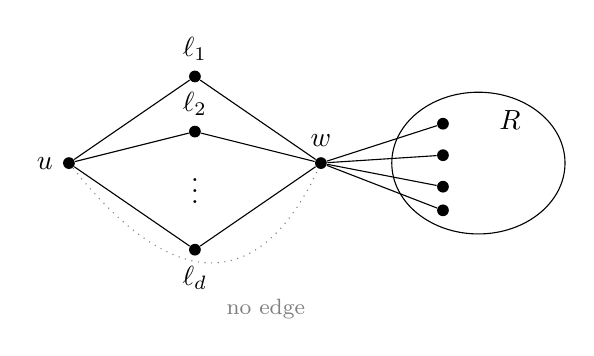
\begin{tikzpicture}[v/.style={circle,fill,inner sep=1.5pt}]
\node[v,label=left:$u$] (u) at (0,0) {};
\node[v,label=above:$\ell_1$] (l1) at (1.6,1.1) {};
\node[v,label=above:$\ell_2$] (l2) at (1.6,0.4) {};
\node at (1.6,-0.25) {$\vdots$};
\node[v,label=below:$\ell_d$] (ld) at (1.6,-1.1) {};
\node[v,label=above:$w$] (w) at (3.2,0) {};
\draw (5.2,0) ellipse (1.1 and 0.9);
\node at (5.6,0.55) {$R$};
\foreach \y [count=\i] in {0.5,0.1,-0.3,-0.6} {\node[v] (r\i) at (4.75,\y) {}; \draw (w)--(r\i);}
\foreach \l in {l1,l2,ld} {\draw (u)--(\l)--(w);}
\draw[dotted,gray] (u) .. controls (1.6,-2.0) and (2.6,-1.3) .. (w);
\node[gray] at (2.5,-1.85) {\footnotesize no edge};
\end{tikzpicture}
\caption{The near-cone $N(d,R)$. The vertex $w$ is joined to $\ell_1,\dots,\ell_d$ and to every vertex of $R$; the centre $u$ of the star is joined only to the leaves $\ell_t$.}
\label{fig:nearcone}
\end{figure}

\begin{lemma}\label{lem:threerules}
Let $m\ge1$.
\begin{enumerate}
\item[\textup{(U)}] If $x\in V_a$ and $y\in\Lam_{m-a}$ with $1\le a\le m$, then $x+y\in\Lam_m$. In particular $1+\Lam_{m-1}\subseteq\Lam_m$.
\item[\textup{(C)}] $2^{m-1}+\Lam_{m-1}\subseteq V_m$.
\item[\textup{(N)}] If $d\ge1$, $r\ge0$ and $d+r+2=m$, then $2^{m-1}-2^r+2^d+d+\Lam_r\subseteq V_m$. More precisely,
\[
c(N(d,R))=2^{m-1}-2^r+2^d+d+c(R).
\]
\end{enumerate}
\end{lemma}

\begin{proof}
(U) is Lemma~\ref{lem:rules}(a); for the second statement add an isolated vertex. (C) is Lemma~\ref{lem:rules}(d).

For (N), let $G'$ be the cone with apex $w$ over $K_{1,d}\sqcup R$. By Lemma~\ref{lem:rules}(a),(d) and Example~\ref{ex:formulas}(i), $c(G')=2^{m-1}+2^d+d+c(R)$. Now remove the edge $wu$ to obtain $G=N(d,R)$. Sets avoiding $w$ or $u$ are connected in $G$ exactly when they are connected in $G'$. A set $\{w\}\cup U$ with $u\in U$ is connected in $G'$. It is disconnected in $G$ exactly when $U$ contains no leaf $\ell_t$, since $u$ is adjacent only to the leaves and every other vertex of $U$ is adjacent to $w$. There are $2^r$ such sets $U$: they contain $u$, no leaf, and an arbitrary set of vertices of $R$. Hence $c(G)=c(G')-2^r$. This is also the case $K=K_{1,d}\sqcup R$ of Lemma~\ref{lem:rules}(e).
\end{proof}

\subsection{Seven sporadic graphs}

\begin{lemma}\label{lem:sporadic}
The seven graphs of Table~\ref{tab:sporadic} and Figure~\ref{fig:sporadic} have the stated values. Hence $19\in V_5$; $25,32,35,57\in V_6$; and $67,90\in V_7$.
\end{lemma}

\begin{table}[ht]
\centering
\small
\begin{tabular}{r c p{7.3cm} p{4.6cm}}
\toprule
$c$ & $m$ & graph & count\\
\midrule
19 & 5 & triangle $xyz$ with one pendant vertex at $x$ and one at $y$ & Ex.~\ref{ex:formulas}(ii): $3\cdot3\cdot2-1+2$\\
32 & 6 & triangle $xyz$ with two pendant vertices at $x$ and one at $y$ & Ex.~\ref{ex:formulas}(ii): $5\cdot3\cdot2-1+3$\\
35 & 6 & diamond $K_4-ab$, with one pendant vertex at $a$ and one at a vertex $z$ of degree $3$ & see the proof\\
57 & 6 & $K_6$ minus two disjoint paths with three vertices each & Ex.~\ref{ex:formulas}(iii): $63-3-3$\\
67 & 7 & $K_{2,3}$ with two pendant vertices at a vertex $x$ of the larger side & Lem.~\ref{lem:rules}(c): $13\cdot4+13+2$\\
90 & 7 & $K_6$ minus two edges $va$, $vb$, with a pendant vertex at $v$ & Lem.~\ref{lem:rules}(c): $29\cdot2+31+1$\\
\midrule
25 & 6 & spider with legs of lengths $1$, $2$, $2$ & Ex.~\ref{ex:formulas}(i): $2\cdot3\cdot3+1+3+3$\\
\bottomrule
\end{tabular}
\caption{The sporadic graphs, drawn in Figure~\ref{fig:sporadic}. The six graphs above the line fill the gaps left by the rules (U), (C) and (N) in Lemma~\ref{lem:base} (Remark~\ref{rem:sharpbase}). The spider below the line realizes $25$ on six vertices.}
\label{tab:sporadic}
\end{table}

\begin{figure}[ht]
\centering
\begin{minipage}[b]{0.24\textwidth}\centering
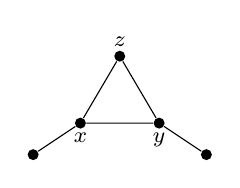
\begin{tikzpicture}[scale=1.0,v/.style={circle,fill,inner sep=1.4pt}]
\node[v] (x) at (0.000,0.000) {};
\node[v] (y) at (1.000,0.000) {};
\node[v] (z) at (0.500,0.850) {};
\node[v] (p1) at (-0.600,-0.400) {};
\node[v] (p2) at (1.600,-0.400) {};
\draw (x)--(y) (x)--(z) (y)--(z) (x)--(p1) (y)--(p2);
\node[below] at (x) {\footnotesize$x$};
\node[below] at (y) {\footnotesize$y$};
\node[above] at (z) {\footnotesize$z$};
\end{tikzpicture}
\\[2pt]{\small $c=19$, $m=5$}
\end{minipage}\hfill
\begin{minipage}[b]{0.24\textwidth}\centering
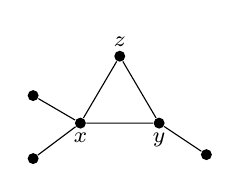
\begin{tikzpicture}[scale=1.0,v/.style={circle,fill,inner sep=1.4pt}]
\node[v] (x) at (0.000,0.000) {};
\node[v] (y) at (1.000,0.000) {};
\node[v] (z) at (0.500,0.850) {};
\node[v] (p1) at (-0.600,-0.450) {};
\node[v] (p2) at (-0.600,0.350) {};
\node[v] (p3) at (1.600,-0.400) {};
\draw (x)--(y) (x)--(z) (y)--(z) (x)--(p1) (x)--(p2) (y)--(p3);
\node[below] at (x) {\footnotesize$x$};
\node[below] at (y) {\footnotesize$y$};
\node[above] at (z) {\footnotesize$z$};
\end{tikzpicture}
\\[2pt]{\small $c=32$, $m=6$}
\end{minipage}\hfill
\begin{minipage}[b]{0.24\textwidth}\centering
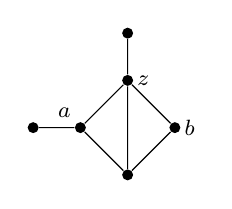
\begin{tikzpicture}[scale=1.0,v/.style={circle,fill,inner sep=1.4pt}]
\node[v] (a) at (0.000,0.500) {};
\node[v] (b) at (1.200,0.500) {};
\node[v] (z) at (0.600,1.100) {};
\node[v] (t) at (0.600,-0.100) {};
\node[v] (pa) at (-0.600,0.500) {};
\node[v] (pz) at (0.600,1.700) {};
\draw (a)--(z) (a)--(t) (b)--(z) (b)--(t) (z)--(t) (a)--(pa) (z)--(pz);
\node[above left] at (a) {\footnotesize$a$};
\node[right] at (b) {\footnotesize$b$};
\node[right] at (z) {\footnotesize$z$};
\end{tikzpicture}
\\[2pt]{\small $c=35$, $m=6$}
\end{minipage}\hfill
\begin{minipage}[b]{0.24\textwidth}\centering
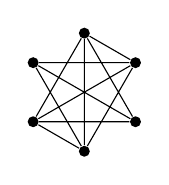
\begin{tikzpicture}[scale=1.0,v/.style={circle,fill,inner sep=1.4pt}]
\node[v] (h0) at (0.000,0.750) {};
\node[v] (h1) at (-0.650,0.375) {};
\node[v] (h2) at (-0.650,-0.375) {};
\node[v] (h3) at (-0.000,-0.750) {};
\node[v] (h4) at (0.650,-0.375) {};
\node[v] (h5) at (0.650,0.375) {};
\draw (h0)--(h2) (h0)--(h3) (h0)--(h4) (h0)--(h5) (h1)--(h3) (h1)--(h4) (h1)--(h5) (h2)--(h3) (h2)--(h4) (h2)--(h5) (h3)--(h5);
\end{tikzpicture}
\\[2pt]{\small $c=57$, $m=6$}
\end{minipage}
\\[10pt]
\begin{minipage}[b]{0.24\textwidth}\centering
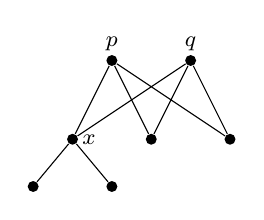
\begin{tikzpicture}[scale=1.0,v/.style={circle,fill,inner sep=1.4pt}]
\node[v] (p) at (0.300,1.000) {};
\node[v] (q) at (1.300,1.000) {};
\node[v] (x) at (-0.200,0.000) {};
\node[v] (y) at (0.800,0.000) {};
\node[v] (w) at (1.800,0.000) {};
\node[v] (s1) at (-0.700,-0.600) {};
\node[v] (s2) at (0.300,-0.600) {};
\draw (p)--(x) (p)--(y) (p)--(w) (q)--(x) (q)--(y) (q)--(w) (x)--(s1) (x)--(s2);
\node[above] at (p) {\footnotesize$p$};
\node[above] at (q) {\footnotesize$q$};
\node[right] at (x) {\footnotesize$x$};
\end{tikzpicture}
\\[2pt]{\small $c=67$, $m=7$}
\end{minipage}\hfill
\begin{minipage}[b]{0.24\textwidth}\centering
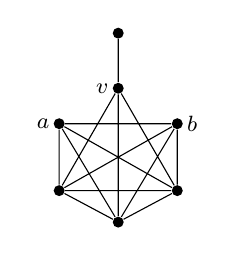
\begin{tikzpicture}[scale=1.0,v/.style={circle,fill,inner sep=1.4pt}]
\node[v] (v) at (0.000,0.850) {};
\node[v] (a) at (-0.750,0.400) {};
\node[v] (b) at (0.750,0.400) {};
\node[v] (c) at (-0.750,-0.450) {};
\node[v] (d) at (0.000,-0.850) {};
\node[v] (e) at (0.750,-0.450) {};
\node[v] (pv) at (0.000,1.550) {};
\draw (v)--(c) (v)--(d) (v)--(e) (a)--(b) (a)--(c) (a)--(d) (a)--(e) (b)--(c) (b)--(d) (b)--(e) (c)--(d) (c)--(e) (d)--(e) (v)--(pv);
\node[left] at (v) {\footnotesize$v$};
\node[left] at (a) {\footnotesize$a$};
\node[right] at (b) {\footnotesize$b$};
\end{tikzpicture}
\\[2pt]{\small $c=90$, $m=7$}
\end{minipage}\hfill
\begin{minipage}[b]{0.24\textwidth}\centering
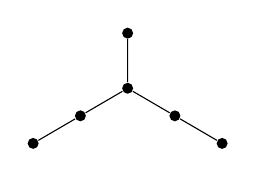
\begin{tikzpicture}[scale=1.0,v/.style={circle,fill,inner sep=1.4pt}]
\node[v] (o) at (0.000,0.000) {};
\node[v] (l1) at (0.000,0.700) {};
\node[v] (m1) at (-0.600,-0.350) {};
\node[v] (m2) at (-1.200,-0.700) {};
\node[v] (n1) at (0.600,-0.350) {};
\node[v] (n2) at (1.200,-0.700) {};
\draw (o)--(l1) (o)--(m1) (m1)--(m2) (o)--(n1) (n1)--(n2);
\end{tikzpicture}
\\[2pt]{\small $c=25$, $m=6$}
\end{minipage}
\caption{The seven sporadic graphs of Table~\ref{tab:sporadic}, with their values of $c$ and their numbers $m$ of vertices. In the graph with $c=57$, the hexagon is drawn without four of its sides; these form the two removed paths with three vertices each.}
\label{fig:sporadic}
\end{figure}

\begin{proof}
The values $19$, $25$, $32$ and $57$ follow from Example~\ref{ex:formulas}; for $57$, $\Phi$ consists of two copies of $K_{1,2}$.

For $c=35$: a connected set is either one of the two pendant vertices, or a connected set $Q$ of the diamond $K_4-ab$ together with any of the pendant vertices attached at $Q$. The connected sets of $K_4-ab$ are all nonempty subsets of its vertex set other than $\{a,b\}$. Summing $2^{|Q\cap\{a,z\}|}$ over all nonempty $Q$ gives $3\cdot3\cdot2\cdot2-1=35$. Removing $Q=\{a,b\}$ subtracts $2$, and the pendant vertices add $2$, giving $35$.

For $c=67$: glue $K_{2,3}$ and the star $K_{1,2}$ at $x$ (Lemma~\ref{lem:rules}(c)). Let $\{p,q\}$ be the smaller side and $\{x,y,z\}$ the larger one. The connected sets of $K_{2,3}$ containing $x$ are $\{x\}$ and the sets $\{x\}\cup S\cup S'$ with $\emptyset\ne S\subseteq\{p,q\}$ and $S'\subseteq\{y,z\}$; there are $1+3\cdot4=13$. Also $K_{2,3}-x=C_4$ has $c=13$, and the star contributes $c_x=4$ and $c(K_{1,2}-x)=2$.

For $c=90$: let $H=K_6-va-vb$ and glue $H$ with an edge at $v$. In $H$, the sets containing $v$ that are disconnected are $\{v,a\}$, $\{v,b\}$ and $\{v,a,b\}$, so $c_v(H)=32-3=29$; and $H-v=K_5$ has $c=31$. The edge contributes $c_v=2$ and $1$.
\end{proof}

\subsection{The base}

\begin{lemma}\label{lem:base}
\begin{enumerate}[label=\textup{(\alph*)}]
\item $\Lam_5\supseteq[5,24]\cup[26,31]$, $\Lam_6\supseteq[6,25]\cup[27,63]$ and $\Lam_7\supseteq[7,127]$.
\item $V_5\supseteq[17,24]\cup[26,31]$, $V_6\supseteq[32,63]$ and $V_7\supseteq[64,127]$.
\end{enumerate}
\end{lemma}

\begin{proof}
We apply the rules of Lemma~\ref{lem:threerules} one order at a time, starting from Lemma~\ref{lem:upto4} and $\Lam_0=\{0\}$. At each order we use only the inclusions already established at smaller orders, and we record only inclusions. We give the order $m=5$ in full; Table~\ref{tab:base} lists every order, including $m\le4$, where the rules reproduce Lemma~\ref{lem:upto4}.

For $m=5$, the rule (C) applied to $\Lam_4=[4,8]\cup[10,15]$ gives $16+\Lam_4=[20,24]\cup[26,31]$. The rule (N) with $(d,r)=(1,2)$ gives $2^4-2^2+2^1+1+\Lam_2=15+\{2,3\}=\{17,18\}$. The sporadic graph with $c=19$ (Lemma~\ref{lem:sporadic}) supplies the remaining value, so $V_5\supseteq[17,24]\cup[26,31]$. By (U), $1+\Lam_4=[5,9]\cup[11,16]$ and $7+3=10\in V_3+\Lam_2$ lie in $\Lam_5$. Together with $V_5$, this gives $\Lam_5\supseteq[5,24]\cup[26,31]$.
\end{proof}

\begin{table}[ht]
\centering
\footnotesize
\newcolumntype{P}[1]{>{\raggedright\arraybackslash}p{#1}}
\begin{tabular}{c P{3.0cm} P{3.7cm} c P{1.7cm} P{3.4cm}}
\toprule
$m$ & cones (C) & near-cones (N), with $(d,r)$ & sporadic & $V_m\supseteq$ & $\Lam_m\supseteq$ by (U) and $V_m$\\
\midrule
2 & $2+\{1\}=\{3\}$ & --- & --- & $\{3\}$ & $1+\{1\}$; so $\{2,3\}$\\
3 & $4+\{2,3\}=\{6,7\}$ & --- & --- & $\{6,7\}$ & $1+\{2,3\}$; so $\{3,4,6,7\}$\\
4 & $8+\{3,4,6,7\}=\{11,12,14,15\}$ & $(1,1)$: $10$; $(2,0)$: $13$ & --- & $[10,15]$ & $1+\{3,4,6,7\}$, $3+3$; so $[4,8]\cup[10,15]$\\
5 & $16+\Lam_4$: $[20,24]\cup[26,31]$ & $(1,2)$: $15+\{2,3\}=\{17,18\}$ & $19$ & $[17,24]\cup[26,31]$ & $[5,9]\cup[11,16]$, $7+3$; so $[5,24]\cup[26,31]$\\
6 & $32+\Lam_5$: $[37,56]\cup[58,63]$ & $(1,3)$: $27+\{3,4,6,7\}=\{30,31,33,34\}$; $(2,2)$: $34+\{2,3\}=\{36,37\}$ & $32,35,57$ & $[32,63]$ & $[6,25]\cup[27,32]$; so $[6,25]\cup[27,63]$\\
7 & $64+\Lam_6$: $[70,89]\cup[91,127]$ & $(1,4)$: $51+[13,15]=[64,66]$; $(2,3)$: $62+\{6,7\}=\{68,69\}$ & $67,90$ & $[64,127]$ & $[7,26]\cup[28,64]$, $24+3$; so $[7,127]$\\
\bottomrule
\end{tabular}
\caption{The steps of the proof of Lemma~\ref{lem:base}. In the cone and near-cone columns, $\Lam_r$ stands for the part of $\Lam_r$ established in the previous rows. The last column lists $1+\Lam_{m-1}$ and the sums $x+y$ with $x\in V_a$, $y\in\Lam_{m-a}$ that are needed, for instance $3+3\in V_2+\Lam_2$ and $24+3\in V_5+\Lam_2$.}
\label{tab:base}
\end{table}

\begin{remark}\label{rem:sharpbase}
Two statements must be distinguished here: a value may fail to be produced by the rules (C) and (N), and a value may fail to be realized by any graph. Lemma~\ref{lem:base} is sharp in the second sense. Indeed $25\notin\Lam_5$, because $25\notin V_5$ (Proposition~\ref{prop:V5}) and a disconnected graph with five vertices has $c\le15+1$. Also $26\notin\Lam_6$, by the computation of Section~\ref{sec:computation}. In the first sense, even with every sporadic graph of smaller order available, the rules (C) and (N) produce on five vertices every value in $[17,31]$ except $19$ and $25$, on six vertices every value in $[32,63]$ except $32$, $35$ and $57$, and on seven vertices every value in $[64,127]$ except $67$ and $90$ (Section~\ref{sec:computation}). All these values except $25$ do lie in $V_m$, and the six sporadic graphs above the line in Table~\ref{tab:sporadic} realize them.
\end{remark}

\subsection{The induction}

\begin{theorem}\label{thm:dyadic}
For every $m\ge8$:
\begin{enumerate}
\item[$(\mathrm G_m)$] $V_m\supseteq[2^{m-1},2^m-1]$;
\item[$(\mathrm H_m)$] $\Lam_m\supseteq[m,2^m-1]$.
\end{enumerate}
\end{theorem}

The two assertions play different roles. The assertion $(\mathrm H_m)$ provides auxiliary graphs, possibly disconnected, with every count from $m$ to $2^m-1$. The assertion $(\mathrm G_m)$ provides connected graphs for the upper half of the range. We prove $(\mathrm G_m)$ from earlier $(\mathrm H)$-statements, and then obtain $(\mathrm H_m)$ by combining $(\mathrm G_m)$ with the isolated-vertex rule (U). In the proof of $(\mathrm G_m)$ the interval splits as
\[
[2^{m-1},2^m-1]=\underbrace{[2^{m-1},\,2^{m-1}+m-2]}_{\text{near-cones}}\ \cup\ \underbrace{[2^{m-1}+m-1,\,2^m-1]}_{\text{cones}}.
\]

\begin{proof}
We use induction on $m\ge8$. The induction hypothesis is $(\mathrm H_{m'})$ for every $m'$ with $7\le m'<m$; for $m'=7$ this is Lemma~\ref{lem:base}(a). The statements $(\mathrm G_{m'})$ are not used.

\emph{Proof of $(\mathrm G_m)$.} By (C) and $(\mathrm H_{m-1})$, $V_m\supseteq2^{m-1}+[m-1,2^{m-1}-1]=[2^{m-1}+m-1,2^m-1]$. It remains to realize $2^{m-1}+j$ for $0\le j\le m-2$. By (N), a pair $(d,r)$ realizes $2^{m-1}+j$ if it satisfies the following conditions:
\begin{enumerate}[label=\textup{(P\arabic*)}]
\item $d\ge1$, $r\ge0$ and $d+r+2=m$;
\item $x_j\in\Lam_r$, where
\begin{equation}\label{eq:need}
x_j:=2^r-2^d-d+j .
\end{equation}
\end{enumerate}
Indeed, if $R$ is a graph with $r$ vertices and $c(R)=x_j$, then $c(N(d,R))=2^{m-1}-2^r+2^d+d+x_j=2^{m-1}+j$. When $r\ge7$ and $r<m$, the hypothesis $(\mathrm H_r)$ gives $[r,2^r-1]\subseteq\Lam_r$. Then (P2) holds for every $j\in[0,m-2]$ as soon as it holds at the two endpoints, that is, as soon as
\begin{enumerate}[label=\textup{(P\arabic*)},start=3]
\item $x_{m-2}\le2^r-1$, which is equivalent to $2^d+d\ge m-1$, and
\item $x_0\ge r$, which is $2^r-2^d-d\ge r$.
\end{enumerate}
Condition (P3) asks for $d$ large and (P4) for $d$ small compared with $r$. For $m\ge12$ we take the least $d$ satisfying (P3). This keeps $d$ close to $\log_2m$, so that $r=m-2-d$ is large. For $8\le m\le11$ this choice leaves $r\le6$, where $(\mathrm H_r)$ is not available, and we check (P2) directly from Lemmas~\ref{lem:upto4}(b) and~\ref{lem:base}(a), with the parameters of Table~\ref{tab:smallm}.

\begin{table}[ht]
\centering
\small
\begin{tabular}{cccccl}
\toprule
$m$ & $(d,r)$ & $j$ & $x_j=2^r-2^d-d+j$ & $x_j\in\Lam_r$ by & \\
\midrule
$8$ & $(2,4)$ & $0,\dots,5$ & $10,\dots,15$ & $\Lam_4\supseteq[10,15]$ & Lemma~\ref{lem:upto4}(b)\\
$8$ & $(3,3)$ & $6$ & $3$ & $3\in\Lam_3$ & Lemma~\ref{lem:upto4}(b)\\
$9$ & $(2,5)$ & $0,\dots,5$ & $26,\dots,31$ & $\Lam_5\supseteq[26,31]$ & Lemma~\ref{lem:base}(a)\\
$9$ & $(3,4)$ & $6,7$ & $11,12$ & $\Lam_4\supseteq[10,15]$ & Lemma~\ref{lem:upto4}(b)\\
$10$ & $(3,5)$ & $0,\dots,8$, $j\ne4$ & $21,\dots,29$, $\ne25$ & $\Lam_5\supseteq[5,24]\cup[26,31]$ & Lemma~\ref{lem:base}(a)\\
$10$ & $(2,6)$ & $4$ & $62$ & $\Lam_6\supseteq[27,63]$ & Lemma~\ref{lem:base}(a)\\
$11$ & $(3,6)$ & $0,\dots,9$ & $53,\dots,62$ & $\Lam_6\supseteq[27,63]$ & Lemma~\ref{lem:base}(a)\\
\bottomrule
\end{tabular}
\caption{The parameters of the near-cones in the proof of Theorem~\ref{thm:dyadic} for $8\le m\le11$, covering $j=0,\dots,m-2$. For $m=10$ the choice $(3,5)$ fails only at $j=4$, since $25\notin\Lam_5$. The graphs $R$ with $c(R)=x_j$ are those given by the proofs of Lemmas~\ref{lem:upto4} and~\ref{lem:base}.}
\label{tab:smallm}
\end{table}

Now let $m\ge12$, let $d$ be the least integer $d\ge1$ with $2^d+d\ge m-1$, and put $r=m-2-d$, so that (P1) and (P3) hold. Then $d\ge3$, since $2^2+2<11$. If $d=3$, then $m=12$ and $r=7$. If $d\ge4$, minimality of $d$ gives $2^{d-1}+d-1<m-1$, so $r=m-2-d\ge2^{d-1}-1\ge7$ and $r\ge d+1$. In both cases $7\le r\le m-3$ and $r\ge d+1$. For (P4),
\[
x_0=2^r-2^d-d\ge2^r-2^{r-1}-(r-1)=2^{r-1}-r+1\ge r,
\]
because $d\le r-1$ and $2^{r-1}\ge2r-1$ for $r\ge4$. Hence, for every $j$ with $0\le j\le m-2$,
\[
r\le x_0\le x_j\le x_{m-2}=2^r-2^d-d+m-2\le2^r-1,
\]
and $x_j\in[r,2^r-1]\subseteq\Lam_r$ by the induction hypothesis $(\mathrm H_r)$, which applies since $7\le r<m$.

\emph{Proof of $(\mathrm H_m)$.} By (U) and $(\mathrm H_{m-1})$, $\Lam_m\supseteq1+[m-1,2^{m-1}-1]=[m,2^{m-1}]$. By $(\mathrm G_m)$, $\Lam_m\supseteq V_m\supseteq[2^{m-1},2^m-1]$.
\end{proof}

\begin{example}\label{ex:128}
Take $k=128=2^7$. Then $m=8$ and $j=0$, and the proof uses $(d,r)=(2,4)$, with $x_0=2^4-2^2-2=10=c(P_4)$. So the near-cone $N(2,P_4)$, formed by the path $P_4$ and the vertices $u$, $\ell_1$, $\ell_2$, $w$, is a connected graph with $8$ vertices and
\[
c(N(2,P_4))=2^7-2^4+2^2+2+10=128.
\]
Seven vertices are not enough, since then $c\le2^7-1$.
\end{example}

\section{Proofs of the main theorems}\label{sec:proofs}

\begin{proof}[Proof of Theorem~\ref{thm:dyadic-intro}]
(a) For $m=6,7$ this is Lemma~\ref{lem:base}(b), and for $m\ge8$ it is Theorem~\ref{thm:dyadic}. (b) For $m=7$ this is Lemma~\ref{lem:base}(a), and for $m\ge8$ it is Theorem~\ref{thm:dyadic}.
\end{proof}

\begin{proof}[Proof of Theorem~\ref{thm:order}]
Let $k\notin\{2,4,5,8,9,16\}$ and put $m=\lfloor\log_2k\rfloor+1$, so that $2^{m-1}\le k\le2^m-1$. A connected graph with fewer than $m$ vertices has $c\le2^{m-1}-1<k$, by Lemma~\ref{lem:rules}(f). It remains to show that $k\in V_m$ when $k\ne25$, and that $25\in V_6$. If $k\le15$, then $k\in\{1,3,6,7\}\cup[10,15]$ and $k\in V_m$ by Lemma~\ref{lem:upto4}. If $17\le k\le31$ and $k\ne25$, then $m=5$ and $k\in V_5$ by Proposition~\ref{prop:V5}. If $k\ge32$, then $m\ge6$ and $k\in V_m$ by Theorem~\ref{thm:dyadic-intro}(a). Finally $25\notin V_5$ by Proposition~\ref{prop:V5}, and the spider with legs $1$, $2$, $2$ shows $25\in V_6$ (Lemma~\ref{lem:sporadic}). Table~\ref{tab:leastorder} lists the witnesses for the values below $32$, where the order is given by the finite base rather than by the induction.
\end{proof}

\begin{table}[ht]
\centering
\small
\begin{tabular}{lcl}
\toprule
$k$ & least order & a connected graph with $c=k$ of least order\\
\midrule
$1$; $3$ & $1$; $2$ & $K_1$; $K_2$\\
$6$; $7$ & $3$ & $P_3$; $K_3$\\
$10,11,12,13,14,15$ & $4$ & $P_4$, $K_{1,3}$, paw, $C_4$, diamond, $K_4$ (Lemma~\ref{lem:upto4})\\
$[17,24]\cup[26,31]$ & $5$ & Table~\ref{tab:base}, row $m=5$, and Appendix~\ref{app:witnesses}; $19$ is sporadic\\
$25$ & $6$ & the spider with legs $1,2,2$ (Lemma~\ref{lem:sporadic})\\
$k\ge32$ & $\lfloor\log_2k\rfloor+1$ & Lemma~\ref{lem:base}(b) for $m=6,7$; Theorem~\ref{thm:dyadic} and Remark~\ref{rem:algorithm} for $m\ge8$\\
\bottomrule
\end{tabular}
\caption{Least orders and witnesses (Theorem~\ref{thm:order}). For each $k\le31$ the least order is $\lfloor\log_2k\rfloor+1$, except for $k=25$.}
\label{tab:leastorder}
\end{table}

\begin{proof}[Proof of Theorem~\ref{thm:main}]
If $k=c(G)$ for a connected graph $G$, then $k\notin\{2,4,5,8,9,16\}$ by Corollary~\ref{cor:upto16}. Conversely, every positive integer outside this set is a value of $c$ on a connected graph by Theorem~\ref{thm:order}.
\end{proof}

\begin{remark}[An algorithm]\label{rem:algorithm}
The proofs are constructive. For $m\ge7$ and $v\in[m,2^m-1]$, the following recursive procedure returns a graph $\mathrm{Re}(m,v)$ with $m$ vertices and $c=v$, which is connected when $v\ge2^{m-1}$.

\emph{Input:} integers $m\ge7$ and $v\in[m,2^m-1]$, in binary. \emph{Output:} the edge list of $\mathrm{Re}(m,v)$ on the vertices $0,\dots,m-1$.
\begin{enumerate}[label=\textup{(\arabic*)}]
\item If $m=7$, return the graph given by the proof of Lemma~\ref{lem:base}, from a fixed table.
\item If $v<2^{m-1}$, return $\mathrm{Re}(m-1,v-1)$ together with an isolated vertex.
\item If $v\ge2^{m-1}+m-1$, return the cone over $\mathrm{Re}(m-1,v-2^{m-1})$.
\item Otherwise put $j=v-2^{m-1}$, choose $(d,r)$ as in the proof of Theorem~\ref{thm:dyadic} (Table~\ref{tab:smallm} for $8\le m\le11$, the least $d$ with $2^d+d\ge m-1$ for $m\ge12$), and return $N(d,R)$. Here $R=\mathrm{Re}(r,x_j)$ if $r\ge7$, and $R$ is the graph given by the proof of Lemma~\ref{lem:upto4} or Lemma~\ref{lem:base}, from a fixed table, if $r\le6$.
\end{enumerate}
The arguments of the recursive calls are admissible: in (2), $v-1\in[m-1,2^{m-1}-1]$; in (3), $v-2^{m-1}\in[m-1,2^{m-1}-1]$; and in (4), $x_j\in[r,2^r-1]$ by the proof of Theorem~\ref{thm:dyadic}. Each call makes at most one recursive call, with fewer vertices, so there are at most $m-6$ calls. We count bit operations. Apart from its recursive call, a call compares and subtracts integers of at most $m+1$ bits, finds $d$ by at most $\log_2m+1$ trials on integers of $O(\log m)$ bits, and computes $x_j$, using $O(m)$ bit operations in all. It also adds at most $2m$ edges: none in (2), $m-1$ in (3), and $2d+r=m-2+d$ in (4). The graph returned by the recursive call keeps its vertices $0,\dots,m'-1$, and the new vertices receive the next labels, so nothing is relabelled. With vertex labels of $O(\log m)$ bits, the new edges take $O(m\log m)$ bits to write. The tables used in (1) and (4) have constant size. Hence $\mathrm{Re}(m,v)$ is computed with $O(m^2\log m)$ bit operations, and its output, a graph with at most $\binom m2$ edges, has $O(m^2\log m)$ bits. For $k\ge64$, the graph $\mathrm{Re}(m,k)$ with $m=\lfloor\log_2k\rfloor+1\ge7$ is connected, has the least possible number of vertices, and is found with $O(\log^2k\cdot\log\log k)$ bit operations, in particular in time polynomial in $\log k$. For $32\le k\le63$ the procedure does not apply, since $m=6$; a connected graph with six vertices and $c=k$ is given by the proof of Lemma~\ref{lem:base}(b). The procedure cannot simply be extended to $m=6$, because $26\notin\Lam_6$. For example, $c=10^{100}$ is realized on $333$ vertices. Section~\ref{sec:computation} reports a check of this procedure.
\end{remark}

\section{Values on a fixed number of vertices}\label{sec:fixed}

Theorem~\ref{thm:dyadic-intro} describes the upper half $[2^{n-1},2^n-1]$ of the range \eqref{eq:range}. The lower half behaves less regularly. Table~\ref{tab:Vn} gives $V_n$ for $n\le8$. For $n\le5$ the table follows from Lemma~\ref{lem:upto4} and Proposition~\ref{prop:V5}; for $n=6,7,8$ it comes from the computer census of Section~\ref{sec:computation}, which confirms \cite[Remark~3.20]{CORa}.

\begin{table}[ht]
\centering
\small
\begin{tabular}{rrrl}
\toprule
$n$ & $\Tr{n}$ & $2^n-1$ & integers in $[\Tr{n},2^n-1]$ not in $V_n$\\
\midrule
1 & 1 & 1 & ---\\
2 & 3 & 3 & ---\\
3 & 6 & 7 & ---\\
4 & 10 & 15 & ---\\
5 & 15 & 31 & $16$, $25$\\
6 & 21 & 63 & $22$, $23$, $26$\\
7 & 28 & 127 & $29$, $30$, $31$, $35$\\
8 & 36 & 255 & $37$, $38$, $39$, $40$, $43$, $50$, $55$\\
\bottomrule
\end{tabular}
\caption{The sets $V_n$ for $n\le8$. For $n\ge5$, the first $n-4$ missing values are $\Tr{n}+1,\dots,\Tr{n}+n-4$ (Corollary~\ref{cor:gap}).}
\label{tab:Vn}
\end{table}

\begin{proposition}\label{prop:fixed}
Let $n\ge6$. Then $\Tr{n}\in V_n$ and $\Tr{n}+n-3\in V_n$, none of the $n-4$ integers $\Tr{n}+1,\dots,\Tr{n}+n-4$ lies in $V_n$, and every integer in $[2^{n-1},2^n-1]$ lies in $V_n$. In particular, at least $n-4$ integers of $[\Tr{n},2^n-1]$ are not values of $c$ on connected graphs with $n$ vertices, and all of them are smaller than $2^{n-1}$.
\end{proposition}

\begin{proof}
Combine Proposition~\ref{prop:pathgap}, Corollary~\ref{cor:gap} and Theorem~\ref{thm:dyadic-intro}(a).
\end{proof}

So the number of missing values in $[\Tr{n},2^n-1]$ grows at least linearly. For $5\le n\le8$ the missing values are the gap above the path together with one or three further values.

\begin{question}\label{q:Vn}
Determine $V_n$ for all $n$. In particular, is the number of integers in $[\Tr{n},2^n-1]\setminus V_n$ bounded by a linear function of $n$?
\end{question}

\section{Related counts}\label{sec:related}

\subsection{Subtrees}
For a tree $T$, $c(T)$ is the number of subtrees of $T$, and Czabarka, Sz\'ekely and Wagner \cite{CSW} showed that every positive integer outside the set
\begin{align*}
E_T=\{&2,4,5,7,8,9,12,13,14,16,18,19,22,23,26,27,29,\\
&31,33,35,38,39,42,43,46,50,52,54,60,65,68,72,77,89\}
\end{align*}
of $34$ exceptions is the number of subtrees of some tree. Thus allowing cycles reduces the $34$ exceptions for trees to the six exceptions of Theorem~\ref{thm:main}.

\begin{remark}[A computer-assisted route]\label{rem:CSWroute}
The theorem of \cite{CSW} gives a second proof of Theorem~\ref{thm:main}. Every positive integer outside $E_T$ is a value of $c$ on a tree. The elements of $E_T$ other than $2,4,5,8,9,16$ are values of $c$ on connected graphs with at most seven vertices, by Lemma~\ref{lem:upto4} and Appendix~\ref{app:witnesses}. With Corollary~\ref{cor:upto16}, this gives Theorem~\ref{thm:main}. This route relies on the computer-assisted parts of \cite{CSW} and on a census of small graphs, and it gives no information on the number of vertices.
\end{remark}

\subsection{All connected subgraphs}
A \emph{connected subgraph} of $G$ is a connected graph $(V',E')$ with $\emptyset\ne V'\subseteq V(G)$ and $E'\subseteq E(G[V'])$. Let $F(G)$ be the number of connected subgraphs of $G$; Pandey and Patra \cite{PP} call it the subgraph index and study its extremal values. Let $L(G)$ denote the line graph of $G$.

\begin{lemma}\label{lem:F}
Let $G$ be a graph with $n$ vertices.
\begin{enumerate}[label=\textup{(\alph*)}]
\item $F(G)=n+c(L(G))$.
\item $c(G)\le F(G)$, with equality if and only if $G$ is a forest.
\item If $G'$ is obtained from $G$ by adding an edge, then $F(G')>F(G)$.
\end{enumerate}
\end{lemma}

\begin{proof}
(a) The connected subgraphs without edges are the $n$ single vertices. A connected subgraph with a nonempty edge set $E'$ has vertex set $V(E')$, the set of ends of edges of $E'$, and the graph $(V(E'),E')$ is connected if and only if $E'$ is a connected set of $L(G)$.

(b) Each connected set $S$ gives the connected subgraph $G[S]$. If $G$ is a forest, then $G[V']$ is a forest, so a connected spanning subgraph of $G[V']$ must be $G[V']$ itself. If $G$ has a cycle, the cycle minus one of its edges is a connected subgraph that is not induced.

(c) All connected subgraphs of $G$ remain, and the new edge with its two ends is a new one.
\end{proof}

\begin{proposition}\label{prop:F}
A positive integer $k$ equals $F(G)$ for some finite connected graph $G$ if and only if
\[
k\notin E_F=\{2,4,5,7,8,9,12,13,14,16,19,22,23,35,38,39,46\}.
\]
\end{proposition}

\begin{proof}[Proof \textup{(computer-assisted)}]
By Lemma~\ref{lem:F}(b) and \cite{CSW}, every positive integer outside $E_T$ is a value of $F$ on a tree, and $\max E_T=89$. It remains to decide which elements of $E_T$ are values of $F$. We separate the reduction, which is proved, from the finite search, which is a computation.

\emph{Reduction.} Let $G$ be connected with $n$ vertices and $F(G)\le89$. By Lemma~\ref{lem:F}(b) and Lemma~\ref{lem:rules}(f), $\Tr{n}\le c(G)\le F(G)\le89$, so $n\le12$. Let $S$ be a spanning tree of $G$, and add the edges of $E(G)\setminus E(S)$ to $S$ one at a time. This gives connected graphs $S=G_0,G_1,\dots,G_s=G$, each obtained from the previous one by adding one edge. By Lemma~\ref{lem:F}(c), $F(G_0)<F(G_1)<\dots<F(G_s)\le89$, and $F(G_0)=c(S)$ by Lemma~\ref{lem:F}(b). So every connected graph with $F\le89$ is reached from a tree with $c\le89$ and at most $12$ vertices by adding one edge at a time, and every intermediate graph also has $F\le89$. Being reachable in this way does not depend on the labeling, so the search may be carried out up to isomorphism.

\emph{Search.} Level $0$ consists of the trees with at most $12$ vertices and $c\le89$, one from each isomorphism class; all trees are generated by NetworkX \cite{NX}. There are $94$ of them: $1$, $1$, $1$, $2$, $3$, $6$, $11$, $20$, $24$, $17$, $6$ and $2$ trees on $1,2,\dots,12$ vertices, respectively. Level $i+1$ consists of the graphs obtained from a graph of level $i$ by adding one missing edge. A graph is discarded if $F>89$, or if it is isomorphic to a graph found before. The isomorphism test compares Weisfeiler--Lehman hashes and then tests exact isomorphism. Levels $1,2,3,4$ contain $69$, $13$, $1$ and $0$ graphs, so the search stops. It finds $177$ pairwise non-isomorphic connected graphs with $F\le89$. By the reduction, every connected graph with $F\le89$ is isomorphic to one of them, and their values of $F$ are all integers in $[1,89]$ except the elements of $E_F$. The $17$ elements of $E_T\setminus E_F$ are realized by the graphs of Table~\ref{tab:F}. The values of $F$ were computed in two independent ways, by Lemma~\ref{lem:F}(a) and by testing all edge subsets; Section~\ref{sec:computation} describes the programs and the machine-readable list of the $177$ graphs.
\end{proof}

\begin{table}[ht]
\centering
\small
\begin{tabular}{rrl@{\qquad}rrl}
\toprule
$F$ & $n$ & edges & $F$ & $n$ & edges\\
\midrule
18 & 4 & 01 02 03 13 \ (paw) & 54 & 5 & 01 02 03 13 24 34\\
26 & 5 & 01 02 13 24 34 \ ($C_5$) & 60 & 7 & 01 02 12 14 23 45 56\\
27 & 5 & 01 02 12 13 34 & 65 & 8 & 01 02 15 23 34 47 56 67\\
29 & 5 & 01 02 04 13 34 & 68 & 7 & 01 02 05 14 23 45 46\\
31 & 5 & 01 02 03 13 34 & 72 & 7 & 01 02 12 13 15 34 56\\
33 & 4 & 01 02 03 12 13 \ (diamond) & 77 & 7 & 01 02 03 04 15 16 56\\
42 & 6 & 01 02 05 14 23 45 & 89 & 8 & 01 02 13 15 23 24 56 67\\
43 & 6 & 01 02 14 23 25 45 & & & \\
50 & 7 & 01 02 14 23 36 45 56 & & & \\
52 & 6 & 01 02 03 05 14 45 & & & \\
\bottomrule
\end{tabular}
\caption{Connected graphs realizing, as values of $F$, the $17$ subtree exceptions of \cite{CSW} that are values of $F$. Each graph has the least possible number of vertices and, among those, the least number of edges. Vertices are $0,\dots,n-1$, and $ij$ denotes the edge joining $i$ and $j$.}
\label{tab:F}
\end{table}

For instance, $F(C_5)=5+c(C_5)=26$, the paw has $F=4+c(\text{diamond})=18$, and the diamond has $F=4+c(W_4)=4+29=33$, where $W_4$, the cone over $C_4$, is the line graph of the diamond. Unlike Theorem~\ref{thm:main}, Proposition~\ref{prop:F} depends on computer calculations, both through \cite{CSW} and through our search. A proof in the spirit of Section~\ref{sec:large} would be of interest.

\subsection{The topological interpretation}
As explained in Section~\ref{subsec:origin}, Theorem~\ref{thm:main} answers \cite[Question~3.21]{CORa}. Combined with the reduction of \cite{CORa} and a realization of every finite connected graph by copies of the Knaster continuum glued at points, it gives the following result of the companion paper.

\begin{theorem}[{\cite[Theorem~A]{AA2}}]\label{thm:topology}
A positive integer $k$ is the number of regular subcontinua of some metric continuum if and only if $k\notin\{2,4,5,8,9,16\}$. For every $k\ge32$ such a continuum can be chosen as the union of $\lfloor\log_2k\rfloor+1$ copies of the Knaster continuum, any two of which meet in at most one point, and no continuum with exactly $k$ regular subcontinua has fewer minimal regular subcontinua.
\end{theorem}

\section{Formal verification in Lean}\label{sec:lean}

The results of Sections~\ref{sec:rules}--\ref{sec:proofs} and~\ref{sec:fixed} and Lemma~\ref{lem:F} are formalized in Lean~4 \cite{Lean} with Mathlib \cite{Mathlib}, in the library \texttt{ConnectedSets} in the directory \texttt{lean} of the repository \cite{GRep} of this paper. The file \texttt{MANIFEST.txt} there lists the SHA-256 checksums of all files of this version, including the Lean sources and the scripts of Section~\ref{sec:computation}. The toolchain is Lean \texttt{v4.35.0} with Mathlib commit \texttt{6015dbbfc399f4548bafd46f9560ff61595fd328}, both fixed in the files \texttt{lean-toolchain}, \texttt{lakefile.toml} and \texttt{lake-manifest.json}. In the directory \texttt{lean}, the commands
\begin{center}
\texttt{lake exe cache get}\qquad\texttt{lake build}\qquad\texttt{lake env lean CheckAxioms.lean}
\end{center}
download a compiled Mathlib (this step is optional), build the library, and print the axioms of every statement of Table~\ref{tab:lean}. The library has $20$ modules and $4623$ lines. Eleven of them (\texttt{Basic}, \texttt{Defs}, \texttt{Rules}, \texttt{Transport}, \texttt{Checker}, \texttt{Five}, \texttt{Sporadic}, \texttt{Base}, \texttt{Intervals}, \texttt{Induction} and \texttt{Main}; $2201$ lines) are the graph-theoretic part of the formalization written for the companion paper \cite{AA2}, which is in the directory \texttt{lean} of \cite{Rep}. They are copied with the namespace renamed and the comments renumbered, and the scripts in \texttt{lean/gen} regenerate the modules \texttt{Sporadic}, \texttt{Base} and \texttt{Intervals} byte for byte. The other modules are new: \texttt{Gap} and \texttt{Path} (Proposition~\ref{prop:pathgap}), \texttt{Spider}, \texttt{Small} (Lemmas~\ref{lem:rules}(b) and~\ref{lem:upto4}, Corollaries~\ref{cor:gap} and~\ref{cor:upto16}, Propositions~\ref{prop:V5} and~\ref{prop:fixed}, and Theorem~\ref{thm:order} for every $k$), \texttt{Glue} (Lemma~\ref{lem:rules}(c)), \texttt{LineGraph} (Lemma~\ref{lem:F}), \texttt{Extras}, and \texttt{Paper}, which states the results with the numbering of this paper.

For a graph \texttt{G} on a finite type \texttt{V}, the number \texttt{c G} is the number of finite sets \texttt{S} of vertices such that the induced graph \texttt{G.induce S} is connected; Mathlib's notion of a connected graph includes nonemptiness. The statement \texttt{InV m k} says that some connected graph on \texttt{Fin m} has \texttt{c = k}, that is, $k\in V_m$, and \texttt{InLam m k} says $k\in\Lam_m$. Paths, forests and line graphs are Mathlib's \texttt{pathGraph}, \texttt{IsAcyclic} and \texttt{lineGraph}. The number \texttt{F G} counts the pairs $(S,E)$ of a finite set of vertices and a finite set of edges of \texttt{G} with both ends in $S$ such that the graph with vertex set $S$ and edge set $E$ is connected. Two of the statements of the module \texttt{Paper} read as follows; there \texttt{T n} is $\Tr{n}$.
\begin{verbatim}
theorem theorem_1_1 (k : ℕ) (hk : 0 < k) :
    (∃ n, ∃ G : SimpleGraph (Fin n), G.Connected ∧ c G = k) ↔
      k ∉ ({2, 4, 5, 8, 9, 16} : Finset ℕ)

theorem proposition_3_2 (G : SimpleGraph V) (hG : G.Connected) :
    (IsEmpty (pathGraph (Fintype.card V) ≃g G) →
      T (Fintype.card V) + (Fintype.card V - 3) ≤ c G) ∧
    (c G = T (Fintype.card V) ↔ Nonempty (pathGraph (Fintype.card V) ≃g G))
\end{verbatim}

Table~\ref{tab:lean} lists the correspondence between this paper and the module \texttt{Paper}; all its declarations are in the namespace \texttt{ConnectedSets.Paper}.

\begin{table}[ht]
\centering
\small
\begin{tabular}{l>{\raggedright\arraybackslash}p{8.4cm}}
\toprule
this paper & declarations in \texttt{ConnectedSets/Paper.lean}\\
\midrule
Theorems~\ref{thm:main}, \ref{thm:order}, \ref{thm:dyadic-intro} & \texttt{theorem\_1\_1}, \texttt{theorem\_1\_1\_type}, \texttt{theorem\_1\_2}, \texttt{theorem\_1\_3}, \texttt{theorem\_1\_3\_sharp}\\
formulas of Section~\ref{sec:intro} & \texttt{section\_1\_formulas} (path, complete graph, star)\\
Lemma~\ref{lem:rules}(a)--(f) & \texttt{lemma\_2\_1\_a}, \dots, \texttt{lemma\_2\_1\_f}\\
Lemma~\ref{lem:upto4} & \texttt{lemma\_3\_1\_a}, \texttt{lemma\_3\_1\_b}\\
Proposition~\ref{prop:pathgap} & \texttt{proposition\_3\_2}, \texttt{proposition\_3\_2\_spider}\\
Corollaries~\ref{cor:gap}, \ref{cor:upto16}; Proposition~\ref{prop:V5} & \texttt{corollary\_3\_3}, \texttt{corollary\_3\_5}, \texttt{proposition\_3\_4}\\
Lemmas~\ref{lem:threerules}, \ref{lem:sporadic}, \ref{lem:base} & \texttt{lemma\_4\_2}, \texttt{lemma\_4\_3}, \texttt{lemma\_4\_4\_a}, \texttt{lemma\_4\_4\_b}\\
Remark~\ref{rem:sharpbase} ($25\notin\Lam_5$) & \texttt{remark\_4\_5}\\
Theorem~\ref{thm:dyadic}, Example~\ref{ex:128} & \texttt{theorem\_4\_6}, \texttt{example\_4\_7}\\
Proposition~\ref{prop:fixed} & \texttt{proposition\_6\_1}\\
Lemma~\ref{lem:F}(a)--(c) & \texttt{lemma\_7\_2\_a}, \texttt{lemma\_7\_2\_b}, \texttt{lemma\_7\_2\_c}\\
\bottomrule
\end{tabular}
\caption{Correspondence between the results of this paper and the Lean formalization.}
\label{tab:lean}
\end{table}

The formal proofs follow the paper, with four differences.
\begin{enumerate}[label=\textup{(\arabic*)}]
\item Proposition~\ref{prop:pathgap} is proved by a different argument, an induction on connected sets that avoids spanning trees. Call a vertex $y$ of a connected set $S$ an \emph{end} of $S$ if $S$ has exactly one connected subset containing $y$ of each size. An end forces $S$ to have exactly $\Tr{|S|}$ connected subsets, and it gives an enumeration of $S$ in which two vertices are adjacent exactly when they are consecutive. Conversely, if $S$ has exactly $\Tr{|S|}$ connected subsets, then every vertex whose removal leaves $S$ connected is an end. In the induction, remove such a vertex $w$. If $S\setminus\{w\}$ has the minimum number of connected subsets, it is a path, and the intervals of this path that form a connected set together with $w$ give at least $2|S|-3$ connected sets containing $w$, unless $S$ itself has the minimum. Otherwise the induction hypothesis applies to $S\setminus\{w\}$. This gives $c(G)=\Tr{n}$ or $c(G)\ge\Tr{n}+n-3$ for every connected graph $G$ with $n$ vertices, and $c(G)=\Tr{n}$ exactly when $G$ is isomorphic to \texttt{pathGraph n}.
\item In Proposition~\ref{prop:V5} the values $16$ and $25$ are excluded by a kernel computation (\texttt{decide +kernel}) over all $2^{10}$ labeled graphs on five vertices, not by the case analysis of the paper; for $16$ the formalized Corollary~\ref{cor:gap} gives a second proof. The computation uses a bitmask counting procedure proved equal to \texttt{c}. The same procedure checks the counts of the sporadic graphs, the $353$ derivations of Lemma~\ref{lem:base}, the exclusions $5\notin\Lam_3$ and $9\notin\Lam_4$ of Lemma~\ref{lem:upto4} (over all labeled graphs on three and four vertices), and $25\notin\Lam_5$ in Remark~\ref{rem:sharpbase}.
\item Lemma~\ref{lem:rules}(c) is formalized inside one graph: the vertex set is covered by sets $A$ and $B$ with $A\cap B=\{v\}$ and no edge between $A\setminus\{v\}$ and $B\setminus\{v\}$, and $G[A]$ and $G[B]$ play the roles of $G_1$ and $G_2$.
\item Lemma~\ref{lem:rules}(e) and the near-cone formula of Lemma~\ref{lem:threerules} are stated without subtraction, for instance as $c(G)+2^{|K|-1-d}=c(K)+2^{|K|}$, where $d$ is the size of a finite set listing the neighbours of $u$.
\end{enumerate}
Not formalized are the general formulas of Example~\ref{ex:formulas}, whose instances used in the proofs are checked by the kernel; the computer census behind Table~\ref{tab:Vn} for $n=6,7,8$, and with it $26\notin\Lam_6$; the statements of Remark~\ref{rem:sharpbase} about which values the rules produce; the running time in Remark~\ref{rem:algorithm}; Remark~\ref{rem:CSWroute} and Proposition~\ref{prop:F}, which rely on the computer-assisted theorem of \cite{CSW} and on our search; and Appendix~\ref{app:witnesses}. Theorem~\ref{thm:topology} is formalized in the companion formalization \cite{AA2}.

The library uses neither \texttt{sorry} nor \texttt{native\_decide} and declares no axioms. Its $31$ statements in the module \texttt{Paper} depend only on the axioms \texttt{propext}, \texttt{Classical.choice} and \texttt{Quot.sound}, and one of them, \texttt{theorem\_1\_2\_minOrder}, depends on none. We checked the library in four ways, recorded in the file \texttt{CHECKS.txt} of the formalization. It builds from an empty build directory, and a copy of the sources in a fresh directory builds with the same output. The declarations of all modules were replayed through the kernel with \texttt{leanchecker}, and the whole import closure, including Lean core and Mathlib, with \texttt{leanchecker --fresh}. Finally, the statements of \texttt{Paper} were exported together with everything they depend on, $10538$ declarations in all, and checked by the independent type checker \texttt{nanoda}, with only the three axioms above permitted; no errors were reported.

\section{Computational verification}\label{sec:computation}

The proofs of Theorems~\ref{thm:main}--\ref{thm:dyadic-intro} do not use a computer. We checked every explicit finite count in this paper, and the computer-assisted result of \cite{CORa}, with programs written for this purpose. The programs for the census of small graphs, the construction and the subtrees, with their outputs, are in the repository \cite{Rep} of the companion paper; the file \texttt{CHECKS.md} there maps each computational statement of \cite{AA2} to the program that checks it. The scripts for Proposition~\ref{prop:F} and Appendix~\ref{app:witnesses}, the construction program \texttt{construct.py} with its certificate for Lemma~\ref{lem:base}, and the outputs are in the directories \texttt{code} and \texttt{data} of the repository \cite{GRep} of this paper.

\emph{Counting.} We compute $c(G)$ in three ways: by testing all $2^n-1$ nonempty vertex sets; by the ESU enumeration scheme \cite{We}, which lists each connected set once; and by a recurrence over vertex sets. In the recurrence, $g(S)=1$ if $G[S]$ is connected and $g(S)=0$ otherwise. The component of $G[S]$ containing $\min S$ is the only connected set $T\subseteq S$ with $\min S\in T$ and no edge between $T$ and $S\setminus T$. Hence $g(S)=1-\sum g(T)$, the sum running over sets $T\ne S$ with $\min S\in T\subseteq S$ and no edge between $T$ and $S\setminus T$.

\emph{Graphs on at most eight vertices.} Program A takes the graphs on at most seven vertices from the atlas of Read and Wilson \cite{RW}, as distributed with NetworkX \cite{NX}. It extends each of the $1044$ graphs on seven vertices, connected or not, by every nonempty neighbourhood of a new vertex, and removes isomorphic copies in two independent ways. Both give the $11117$ connected graphs on eight vertices of OEIS A001349 \cite{OEIS}. Program B, written in C, uses no atlas and no isomorphism test. It runs over all labeled graphs on at most seven vertices, and over the graphs on eight vertices obtained by extending the labeled graphs on seven vertices with nonincreasing degree sequence. Its numbers of labeled connected graphs agree with OEIS A001187. The two programs give the same sets $V_n$ for $n\le8$, as in Table~\ref{tab:Vn}. Every value in $[1,255]$ except $2,4,5,8,9,16$ occurs, and every value in $[17,127]$ occurs on at most seven vertices. This confirms \cite[Remark~3.20]{CORa}. Program B also rederives each witness of Appendix~\ref{app:witnesses} by brute force over all labeled graphs.

\emph{The construction.} We implemented Lemma~\ref{lem:base} and the procedure of Remark~\ref{rem:algorithm} literally, and checked the gaps stated in Remark~\ref{rem:sharpbase}. An independently written program re-checked each of the $353$ derivations for $m\le7$. For every $k\in[17,70000]$, and for $300$ random $k<2^{22}$, we built the resulting graph and counted its connected sets. For every $8\le m\le16$ and every $v\in[m,2^m-1]$, the graph $\mathrm{Re}(m,v)$ has exactly $m$ vertices, is connected when $v\ge2^{m-1}$, and has $c=v$; in total $130708$ graphs were checked.

\emph{Subtrees.} We re-verified the list $E_T$ of \cite{CSW} from all trees with at most $18$ vertices, generated and counted in two independent ways. A tree with $n\ge19$ vertices has at least $\Tr{19}=190$ subtrees, so this determines the subtree counts below $190$.

\emph{All connected subgraphs.} The script \texttt{code/f\_values.py} of \cite{GRep} carries out the search in the proof of Proposition~\ref{prop:F}; the command \texttt{python3 f\_values.py 89} runs it, with Python~3.13 and NetworkX~3.7, in about two seconds. During the search it computes $F$ through Lemma~\ref{lem:F}(a), counting the connected sets of the line graph with the ESU scheme and stopping as soon as the count exceeds $89$. For every graph found it then recomputes $F$ by testing all nonempty edge subsets with a union-find structure; the two methods agree on all $177$ graphs. The script prints the number of trees of each order at level $0$, the size of each level, and the missing values, as stated in the proof (output file \texttt{f\_values\_output.txt}). It also writes the file \texttt{f\_graphs\_le\_89.csv}, which lists the $177$ graphs with $F$, $c$, the numbers of vertices and edges, and the edge list. Together with the reduction in the proof, this list certifies both that the values in $[1,89]\setminus E_F$ occur and that the elements of $E_F$ do not. A separate program in C, \texttt{f\_edge\_subsets.c}, recomputed $c$ by vertex subsets and $F$ by edge subsets for all $996$ connected graphs with at most seven vertices of the atlas, independently of the search. It agrees with the values below $36$, where those graphs suffice, since $F\ge\Tr{n}\ge36$ for $n\ge8$.

\section*{AI disclosure}

Artificial intelligence was used extensively in this work, both to obtain the results and to check them.

\emph{Solving and proving.} The main model used to solve the problem and to prove the theorems was Claude Opus 5.5 (Anthropic). In an iterative process directed by the author, it carried out most of the exploratory proof development, including the near-cones of Section~\ref{sec:large} and the arguments of Section~\ref{sec:small}. It also wrote and ran the programs of Section~\ref{sec:computation}, carried out the literature search of Section~\ref{subsec:literature}, and generated most of the first draft of this manuscript and of the Lean~4 formalization of Section~\ref{sec:lean}.

\emph{Reading and checking.} ChatGPT-Astra (OpenAI) was used, together with the author, to read the manuscript and check the arguments. AI was used extensively for proofreading and proof checking, and for repeated rounds of checking the arguments and comparing the proofs with one another, for instance the two proofs of Proposition~\ref{prop:pathgap} and the two exclusions of $16$ on five vertices. In each round the author, with ChatGPT-Astra, reviewed the text, the proofs and the supplementary material and sent feedback, and Claude revised them.

\emph{The author's role.} The author formulated the problem, which arose from Questions~3.5 and~3.21 of \cite{CORa}, provided the mathematical context and constraints, and steered the iterations through prompts and feedback. The author also supplied ideas and suggested strategies, selected and revised the outputs, and reviewed the final arguments.

The explicit finite counts are checked by programs (Section~\ref{sec:computation}), and the results listed in Table~\ref{tab:lean} are formally verified in Lean (Section~\ref{sec:lean}). No independent expert has yet verified the proofs. The author takes full responsibility for the content.

\begin{thebibliography}{99}

\bibitem{Mostar}
Y.~Alizadeh, N.~Ba\v{s}i\'c, I.~Damnjanovi\'c, T.~Do\v{s}li\'c, T.~Pisanski, D.~Stevanovi\'c, and K.~Xu,
\emph{Solving the Mostar index inverse problem},
preprint, \arXiv{2312.13083}.

\bibitem{AA2}
L.~Alves de Almeida,
\emph{All finite cardinalities of the hyperspace of regular subcontinua},
preprint, version~2.3, 2026, available in \cite{Rep}.

\bibitem{GRep}
L.~Alves de Almeida,
\emph{The inverse problem for the number of connected induced subgraphs: paper, Lean formalization and programs},
GitHub repository, \grepo.

\bibitem{Rep}
L.~Alves de Almeida,
\emph{All finite cardinalities of the hyperspace of regular subcontinua: paper, programs and Lean formalization},
GitHub repository, \repo.

\bibitem{ADO}
E.~O.~D.~Andriantiana and A.~A.~V.~Dossou-Olory,
\emph{Nordhaus--Gaddum inequalities for the number of connected induced subgraphs in graphs},
preprint, \arXiv{2006.01187}.

\bibitem{BS}
C.~Bernert and J.~Shaw,
\emph{The inverse problem for the Steiner--Wiener index via additive number theory},
preprint, 2026, \arXiv{2603.17559}.

\bibitem{CORa}
J.~Camargo, N.~Ordo\~nez, and D.~Ram\'irez,
\emph{On the hyperspaces of meager and regular continua},
Appl. Gen. Topol. \textbf{25} (2024), no.~2, 385--406.
\doi{10.4995/agt.2024.20116}.

\bibitem{CSW}
\'E.~Czabarka, L.~A.~Sz\'ekely, and S.~Wagner,
\emph{The inverse problem for certain tree parameters},
Discrete Appl. Math. \textbf{157} (2009), no.~15, 3314--3319.
\doi{10.1016/j.dam.2009.07.004}.

\bibitem{Lean}
L.~de~Moura and S.~Ullrich,
\emph{The Lean~4 theorem prover and programming language},
in: Automated Deduction -- CADE~28, Lecture Notes in Comput. Sci. \textbf{12699}, Springer, Cham, 2021, 625--635.
\doi{10.1007/978-3-030-79876-5_37}.

\bibitem{DO1}
A.~A.~V.~Dossou-Olory,
\emph{Graphs and unicyclic graphs with extremal number of connected induced subgraphs},
preprint, \arXiv{1812.02422}.

\bibitem{DO2}
A.~A.~V.~Dossou-Olory,
\emph{Cut and pendant vertices and the number of connected induced subgraphs of a graph},
preprint, \arXiv{1910.04552}.

\bibitem{DO3}
A.~A.~V.~Dossou-Olory,
\emph{On the maximum number of connected induced subgraphs of a graph},
preprint, 2023, \arXiv{2303.01964}.

\bibitem{NX}
A.~A.~Hagberg, D.~A.~Schult, and P.~J.~Swart,
\emph{Exploring network structure, dynamics, and function using NetworkX},
in: Proceedings of the 7th Python in Science Conference (SciPy 2008), 11--15.

\bibitem{Ha}
J.~Haslegrave,
\emph{The number and average size of connected sets in graphs with degree constraints},
preprint, \arXiv{2105.13332}.

\bibitem{Li}
V.~Linek,
\emph{Bipartite graphs can have any number of independent sets},
Discrete Math. \textbf{76} (1989), 131--136.
\doi{10.1016/0012-365X(89)90306-3}.

\bibitem{Mathlib}
The mathlib Community,
\emph{The Lean mathematical library},
in: Proceedings of the 9th ACM SIGPLAN International Conference on Certified Programs and Proofs (CPP 2020), 367--381.
\doi{10.1145/3372885.3373824}.

\bibitem{OEIS}
OEIS Foundation Inc.,
\emph{The On-Line Encyclopedia of Integer Sequences},
sequences A001187 and A001349, \url{https://oeis.org}.

\bibitem{Or18}
N.~Ordo\~nez,
\emph{The hyperspace of regular subcontinua},
Topology Appl. \textbf{234} (2018), 415--427.
\doi{10.1016/j.topol.2017.11.038}.

\bibitem{PP}
D.~Pandey and K.~L.~Patra,
\emph{On the number of connected subgraphs of graphs},
Indian J. Pure Appl. Math. \textbf{52} (2021), no.~2, 571--583.
\doi{10.1007/s13226-021-00061-4}.

\bibitem{RW}
R.~C.~Read and R.~J.~Wilson,
\emph{An Atlas of Graphs},
Oxford University Press, Oxford, 1998.

\bibitem{SW}
L.~A.~Sz\'ekely and H.~Wang,
\emph{On subtrees of trees},
Adv. in Appl. Math. \textbf{34} (2005), 138--155.
\doi{10.1016/j.aam.2004.07.002}.

\bibitem{TAM}
P.~Tittmann, I.~Averbouch, and J.~A.~Makowsky,
\emph{The enumeration of vertex induced subgraphs with respect to the number of components},
European J. Combin. \textbf{32} (2011), no.~7, 954--974.
\doi{10.1016/j.ejc.2011.03.017}.

\bibitem{Vi}
A.~Vince,
\emph{Counting connected sets and connected partitions of a graph},
Australas. J. Combin. \textbf{67} (2017), no.~2, 281--293.

\bibitem{WY}
H.~Wang and G.~Yu,
\emph{All but 49 numbers are Wiener indices of trees},
Acta Appl. Math. \textbf{92} (2006), 15--20.
\doi{10.1007/s10440-006-9037-2}.

\bibitem{We}
S.~Wernicke,
\emph{Efficient detection of network motifs},
IEEE/ACM Trans. Comput. Biol. Bioinform. \textbf{3} (2006), no.~4, 347--359.
\doi{10.1109/TCBB.2006.51}.

\end{thebibliography}

\appendix

\section{Witnesses for the values from 17 to 127}\label{app:witnesses}

A \emph{witness} for an integer $k$ is a connected graph $G$ with $c(G)=k$. We record witnesses as graph6 strings. A \emph{graph6 string} is a standard printable encoding of a finite labeled graph with vertex set $\{0,\dots,n-1\}$. For $n\le62$ its first character is the one with ASCII code $n+63$. The remaining characters encode the entries above the diagonal of the adjacency matrix, read column by column, that is, in the order $(0,1),(0,2),(1,2),(0,3),(1,3),(2,3),\dots$. These bits are padded with zeros to a multiple of six, and each group of six bits, read as a binary number $b$, is written as the character with ASCII code $b+63$. For example, \verb!D?{! encodes the star $K_{1,4}$ with centre $4$: the bits of \verb!?! and \verb!{! are $000000$ and $111100$, so the edges are $(0,4),(1,4),(2,4),(3,4)$.

\emph{Canonical strings.} A graph6 string depends on the labeling. For a fixed $n$ all graph6 strings have the same length, and we compare them lexicographically by their ASCII characters. The \emph{canonical graph6 string} of a graph is the least graph6 string among all its labelings with vertex set $\{0,\dots,n-1\}$; two graphs are isomorphic if and only if their canonical strings coincide.

\emph{Witness rule.} For each $k\in[17,127]$ the table gives a witness of least possible order $n$; among those, of least number of edges; and among those, the one with the least canonical graph6 string. The table lists $k$, $n$ and the canonical string. By Theorem~\ref{thm:order}, $n=\lfloor\log_2k\rfloor+1$ except for $k=25$. Program~B of Section~\ref{sec:computation} rederives every entry by brute force over all labeled graphs on at most seven vertices. Edge lists are in the file \texttt{data/witnesses\_small.csv} of \cite{GRep}. The script \texttt{code/check\_witnesses.py} of \cite{GRep} reads this table from the \LaTeX{} source of the paper, decodes each string with the rule above, and checks that it gives a connected graph with $n$ vertices and exactly $k$ connected sets; all $111$ rows pass.

{\footnotesize
\begin{longtable}{rcl@{\hspace{3em}}rcl@{\hspace{3em}}rcl}
\toprule
$k$ & $n$ & graph6 & $k$ & $n$ & graph6 & $k$ & $n$ & graph6 \\
\midrule
\endfirsthead
\toprule
$k$ & $n$ & graph6 & $k$ & $n$ & graph6 & $k$ & $n$ & graph6 \\
\midrule
\endhead
\bottomrule
\endfoot
17 & 5 & \verb!D@s! & 54 & 6 & \verb!EB~o! & 91 & 7 & \verb!F?Nv_! \\
18 & 5 & \verb!DJc! & 55 & 6 & \verb!EFz_! & 92 & 7 & \verb!F?Fno! \\
19 & 5 & \verb!DBk! & 56 & 6 & \verb!EFzg! & 93 & 7 & \verb!F@Q~o! \\
20 & 5 & \verb!D?{! & 57 & 6 & \verb!EL~o! & 94 & 7 & \verb!F?Fnw! \\
21 & 5 & \verb!D@{! & 58 & 6 & \verb!EFzw! & 95 & 7 & \verb!F?]~_! \\
22 & 5 & \verb!DJk! & 59 & 6 & \verb!EF~w! & 96 & 7 & \verb!F@Vn_! \\
23 & 5 & \verb!DB{! & 60 & 6 & \verb!E]~o! & 97 & 7 & \verb!F@N^W! \\
24 & 5 & \verb!DLs! & 61 & 6 & \verb!E]~w! & 98 & 7 & \verb!F?Nvo! \\
25 & 6 & \verb!E@QW! & 62 & 6 & \verb!E^~w! & 99 & 7 & \verb!F@vf_! \\
26 & 5 & \verb!DFw! & 63 & 6 & \verb!E~~w! & 100 & 7 & \verb!F?B~o! \\
27 & 5 & \verb!DF{! & 64 & 7 & \verb!F?DnO! & 101 & 7 & \verb!F?B~w! \\
28 & 5 & \verb!DN{! & 65 & 7 & \verb!F??^o! & 102 & 7 & \verb!F?F~w! \\
29 & 5 & \verb!D]{! & 66 & 7 & \verb!F?C^W! & 103 & 7 & \verb!F?N~o! \\
30 & 5 & \verb!D^{! & 67 & 7 & \verb!F?KuW! & 104 & 7 & \verb!F?^vo! \\
31 & 5 & \verb!D~{! & 68 & 7 & \verb!F?Cng! & 105 & 7 & \verb!F@^vo! \\
32 & 6 & \verb!E?NW! & 69 & 7 & \verb!F?@|w! & 106 & 7 & \verb!F@vv_! \\
33 & 6 & \verb!E@Ug! & 70 & 7 & \verb!F??Fw! & 107 & 7 & \verb!F?^~o! \\
34 & 6 & \verb!EJ]G! & 71 & 7 & \verb!F??Nw! & 108 & 7 & \verb!FBnnO! \\
35 & 6 & \verb!E@Uw! & 72 & 7 & \verb!F?Cfw! & 109 & 7 & \verb!F@vvo! \\
36 & 6 & \verb!E?No! & 73 & 7 & \verb!F??^w! & 110 & 7 & \verb!FBzv_! \\
37 & 6 & \verb!E?Bw! & 74 & 7 & \verb!F?C^w! & 111 & 7 & \verb!F@vvw! \\
38 & 6 & \verb!E?Fw! & 75 & 7 & \verb!F@Q^G! & 112 & 7 & \verb!F?~v_! \\
39 & 6 & \verb!E@Rw! & 76 & 7 & \verb!F?Cnw! & 113 & 7 & \verb!F?~vg! \\
40 & 6 & \verb!E?Nw! & 77 & 7 & \verb!F??~w! & 114 & 7 & \verb!F@~vg! \\
41 & 6 & \verb!E@Nw! & 78 & 7 & \verb!F?Dno! & 115 & 7 & \verb!F?~vw! \\
42 & 6 & \verb!E?^o! & 79 & 7 & \verb!F@Um_! & 116 & 7 & \verb!F?~~w! \\
43 & 6 & \verb!E@Vw! & 80 & 7 & \verb!F?LVw! & 117 & 7 & \verb!F@~~w! \\
44 & 6 & \verb!E?^w! & 81 & 7 & \verb!F@Q^W! & 118 & 7 & \verb!FFzng! \\
45 & 6 & \verb!E@vg! & 82 & 7 & \verb!F?Dnw! & 119 & 7 & \verb!FFzfw! \\
46 & 6 & \verb!EBn_! & 83 & 7 & \verb!F?@~o! & 120 & 7 & \verb!FFznw! \\
47 & 6 & \verb!E@vo! & 84 & 7 & \verb!F?D~o! & 121 & 7 & \verb!FFz~o! \\
48 & 6 & \verb!EBz_! & 85 & 7 & \verb!F?@~w! & 122 & 7 & \verb!FFz~w! \\
49 & 6 & \verb!E@vw! & 86 & 7 & \verb!F?Fng! & 123 & 7 & \verb!FF~~w! \\
50 & 6 & \verb!EJfw! & 87 & 7 & \verb!F@Umg! & 124 & 7 & \verb!F]~vw! \\
51 & 6 & \verb!E?~o! & 88 & 7 & \verb!F?NNg! & 125 & 7 & \verb!F]~~w! \\
52 & 6 & \verb!E?~w! & 89 & 7 & \verb!F?N^_! & 126 & 7 & \verb!F^~~w! \\
53 & 6 & \verb!E@~w! & 90 & 7 & \verb!F@]v_! & 127 & 7 & \verb!F~~~w! \\
\end{longtable}
}

\end{document}
